% !TeX program = lualatex
\documentclass{article}
\usepackage{graphicx} % Required for inserting images
\usepackage{amsmath}
\usepackage{amsfonts}
\usepackage{amsthm}
\usepackage{amssymb}
\usepackage{float}
\usepackage{hyperref}
\usepackage{amssymb}
\usepackage{unicode-math}
\usepackage{colortbl}     % for \rowcolor
\usepackage{xcolor}       % for \definecolor
\usepackage{microtype}
\usepackage{booktabs}
\usepackage{array}
\usepackage{caption}
\usepackage{tikz}
\usetikzlibrary{shapes, arrows, intersections, bending}

\definecolor{headerblue}{RGB}{30, 80, 140}
\definecolor{rowlight}{RGB}{235, 242, 252}
\definecolor{rowwhite}{RGB}{255, 255, 255}
\setmainfont{Latin Modern Roman}
\setmathfont{STIX Two Math} % <-- important

\theoremstyle{plain}   % <-- this keeps headings left-aligned
\newtheorem{theorem}{Theorem}
\newtheorem{lemma}{Lemma}
\newtheorem{remark}{Remark}
\newtheorem{conjecture}{Conjecture}
\newtheorem{corollary}{Corollary}
\newtheorem{proposition}{Proposition}
\newtheorem{definition}{Definition}
\newtheorem{example}{Example}

\newcommand{\extendR}{\overline{\mathbb{R}}}
\newcommand{\infcomp}{\overset{\rightharpoonup}{\circ}}
\newcommand{\supcomp}{\overset{\rightharpoondown}{\circ}}
\newcommand{\rtop}{\rotatebox{90}{$\top$}}
\newcommand{\llbracket}{[\![}
\newcommand{\rrbracket}{]\!]}
\newcommand{\mushroom}{⫏-}
\renewcommand{\arraystretch}{1.8}

\usepackage[
backend=biber,
style=alphabetic,
]{biblatex}
\bibliography{../bib.bib}

% Every pic occupies the uniform frame x in [-0.5, 0.5], y in [-0.5, 0.5].
% Tips live on the left/right edges as (-in-k) / (-out-k), top-first,
% evenly spaced in [-0.5, 0.5]: for n tips, y_k = 0.5 - k/(n-1) (n >= 2),
% or y_0 = 0 when n = 1. Codegen relies on this convention to align tips
% across composition without needing tip data in JSON.
%
% Coloured node glyphs (whitedot / boxnode_*) are drawn *after* the wires so
% the fill covers any wire segment passing through the node interior.
\tikzset{
  val/.store in = \argval,
  multiplication/.pic = {
    \coordinate (-in-0)  at (-0.5, 0.5);
    \coordinate (-in-1)  at (-0.5,-0.5);
    \coordinate (-out-0) at ( 0.5, 0);
    \draw (-in-0) to[bend left=20]  (0,0);
    \draw (-in-1) to[bend right=20] (0,0);
    \draw (0,0)   to (-out-0);
    \node[whitedot] (-node) at (0,0) {};
  },
  comultiplication/.pic = {
    \coordinate (-in-0)  at (-0.5, 0);
    \coordinate (-out-0) at ( 0.5, 0.5);
    \coordinate (-out-1) at ( 0.5,-0.5);
    \draw (-in-0) to (0,0);
    \draw (0,0)   to[bend left=20]  (-out-0);
    \draw (0,0)   to[bend right=20] (-out-1);
    \node[whitedot] (-node) at (0,0) {};
  },
  zero/.pic = {
    \coordinate (-out-0) at (0.5, 0);
    \draw (0,0) to (-out-0);
    \node[whitedot] (-node) at (0,0) {};
  },
  cozero/.pic = {
    \coordinate (-in-0) at (-0.5, 0);
    \draw (-in-0) to (0,0);
    \node[whitedot] (-node) at (0,0) {};
  },
  copy/.pic = {
    \coordinate (-in-0)  at (-0.5, 0);
    \coordinate (-out-0) at ( 0.5, 0.5);
    \coordinate (-out-1) at ( 0.5,-0.5);
    \draw (-in-0) to (0,0);
    \draw (0,0)   to[bend left=20]  (-out-0);
    \draw (0,0)   to[bend right=20] (-out-1);
    \node[blackdot] (-node) at (0,0) {};
  },
  cocopy/.pic = {
    \coordinate (-in-0)  at (-0.5, 0.5);
    \coordinate (-in-1)  at (-0.5,-0.5);
    \coordinate (-out-0) at ( 0.5, 0);
    \draw (-in-0) to[bend left=20]  (0,0);
    \draw (-in-1) to[bend right=20] (0,0);
    \draw (0,0)   to (-out-0);
    \node[blackdot] (-node) at (0,0) {};
  },
  discard/.pic = {
    \coordinate (-in-0) at (-0.5, 0);
    \draw (-in-0) to (0,0);
    \node[blackdot] (-node) at (0,0) {};
  },
  codiscard/.pic = {
    \coordinate (-out-0) at (0.5, 0);
    \draw (0,0) to (-out-0);
    \node[blackdot] (-node) at (0,0) {};
  },
  scalar/.pic = {
    \coordinate (-in-0)  at (-0.5, 0);
    \coordinate (-out-0) at ( 0.5, 0);
    \draw (-in-0) to (0,0);
    \draw (0,0)   to (-out-0);
    \node[boxnode_right] (-node) at (0,0) {$\argval$};
  },
  coscalar/.pic = {
    \coordinate (-in-0)  at (-0.5, 0);
    \coordinate (-out-0) at ( 0.5, 0);
    \draw (-in-0) to (0,0);
    \draw (0,0)   to (-out-0);
    \node[boxnode_left] (-node) at (0,0) {$\argval$};
  },
  matrix/.pic = {
    \coordinate (-in-0)  at (-0.5, 0);
    \coordinate (-out-0) at ( 0.5, 0);
    \draw (-in-0) to (0,0);
    \draw (0,0)   to (-out-0);
    \node[matrixnode_right] (-node) at (0,0) {$\argval$};
  },
  comatrix/.pic = {
    \coordinate (-in-0)  at (-0.5, 0);
    \coordinate (-out-0) at ( 0.5, 0);
    \draw (-in-0) to (0,0);
    \draw (0,0)   to (-out-0);
    \node[matrixnode_left] (-node) at (0,0) {$\argval$};
  },
  relation/.pic = {
    \coordinate (-in-0)  at (-0.5, 0);
    \coordinate (-out-0) at ( 0.5, 0);
    \draw (-in-0) to (0,0);
    \draw (0,0)   to (-out-0);
    \node[relationnode_right] (-node) at (0,0) {$\argval$};
  },
  corelation/.pic = {
    \coordinate (-in-0)  at (-0.5, 0);
    \coordinate (-out-0) at ( 0.5, 0);
    \draw (-in-0) to (0,0);
    \draw (0,0)   to (-out-0);
    \node[relationnode_left] (-node) at (0,0) {$\argval$};
  },
  affine/.pic = {
    \coordinate (-out-0) at (0.5, 0);
    \draw (0,0) to (-out-0);
    \node (-node) at (0,0) {$|$};
  },
  ge/.pic = {
    \coordinate (-in-0)  at (-0.5, 0);
    \coordinate (-out-0) at ( 0.5, 0);
    \draw (-in-0) to (0,0);
    \draw (0,0)   to (-out-0);
    \node[boxnode_right] (-node) at (0,0) {$\ge$};
  },
  coge/.pic = {
    \coordinate (-in-0)  at (-0.5, 0);
    \coordinate (-out-0) at ( 0.5, 0);
    \draw (-in-0) to (0,0);
    \draw (0,0)   to (-out-0);
    \node[boxnode_left] (-node) at (0,0) {$\le$};
  },
  linear/.pic = {
    \coordinate (-out-0) at (0.5, 0);
    \draw (0,0) to (-out-0);
    \node[leftseminode] (-node) at (0,0) {};
  }
}

% Every pic occupies the uniform frame x in [-0.5, 0.5], y in [-0.5, 0.5].
% Tips live on the left/right edges as (-in-k) / (-out-k), top-first,
% evenly spaced in [-0.5, 0.5]: for n tips, y_k = 0.5 - k/(n-1) (n >= 2),
% or y_0 = 0 when n = 1. Codegen relies on this convention to align tips
% across composition without needing tip data in JSON.
%
% Coloured node glyphs (whitedot / boxnode_*) are drawn *after* the wires so
% the fill covers any wire segment passing through the node interior.
\tikzset{
  val/.store in = \argval,
  multiplication/.pic = {
    \coordinate (-in-0)  at (-0.5, 0.5);
    \coordinate (-in-1)  at (-0.5,-0.5);
    \coordinate (-out-0) at ( 0.5, 0);
    \draw (-in-0) to[bend left=20]  (0,0);
    \draw (-in-1) to[bend right=20] (0,0);
    \draw (0,0)   to (-out-0);
    \node[whitedot] (-node) at (0,0) {};
  },
  comultiplication/.pic = {
    \coordinate (-in-0)  at (-0.5, 0);
    \coordinate (-out-0) at ( 0.5, 0.5);
    \coordinate (-out-1) at ( 0.5,-0.5);
    \draw (-in-0) to (0,0);
    \draw (0,0)   to[bend left=20]  (-out-0);
    \draw (0,0)   to[bend right=20] (-out-1);
    \node[whitedot] (-node) at (0,0) {};
  },
  zero/.pic = {
    \coordinate (-out-0) at (0.5, 0);
    \draw (0,0) to (-out-0);
    \node[whitedot] (-node) at (0,0) {};
  },
  cozero/.pic = {
    \coordinate (-in-0) at (-0.5, 0);
    \draw (-in-0) to (0,0);
    \node[whitedot] (-node) at (0,0) {};
  },
  copy/.pic = {
    \coordinate (-in-0)  at (-0.5, 0);
    \coordinate (-out-0) at ( 0.5, 0.5);
    \coordinate (-out-1) at ( 0.5,-0.5);
    \draw (-in-0) to (0,0);
    \draw (0,0)   to[bend left=20]  (-out-0);
    \draw (0,0)   to[bend right=20] (-out-1);
    \node[blackdot] (-node) at (0,0) {};
  },
  cocopy/.pic = {
    \coordinate (-in-0)  at (-0.5, 0.5);
    \coordinate (-in-1)  at (-0.5,-0.5);
    \coordinate (-out-0) at ( 0.5, 0);
    \draw (-in-0) to[bend left=20]  (0,0);
    \draw (-in-1) to[bend right=20] (0,0);
    \draw (0,0)   to (-out-0);
    \node[blackdot] (-node) at (0,0) {};
  },
  discard/.pic = {
    \coordinate (-in-0) at (-0.5, 0);
    \draw (-in-0) to (0,0);
    \node[blackdot] (-node) at (0,0) {};
  },
  codiscard/.pic = {
    \coordinate (-out-0) at (0.5, 0);
    \draw (0,0) to (-out-0);
    \node[blackdot] (-node) at (0,0) {};
  },
  scalar/.pic = {
    \coordinate (-in-0)  at (-0.5, 0);
    \coordinate (-out-0) at ( 0.5, 0);
    \draw (-in-0) to (0,0);
    \draw (0,0)   to (-out-0);
    \node[boxnode_right] (-node) at (0,0) {$\argval$};
  },
  coscalar/.pic = {
    \coordinate (-in-0)  at (-0.5, 0);
    \coordinate (-out-0) at ( 0.5, 0);
    \draw (-in-0) to (0,0);
    \draw (0,0)   to (-out-0);
    \node[boxnode_left] (-node) at (0,0) {$\argval$};
  },
  matrix/.pic = {
    \coordinate (-in-0)  at (-0.5, 0);
    \coordinate (-out-0) at ( 0.5, 0);
    \draw (-in-0) to (0,0);
    \draw (0,0)   to (-out-0);
    \node[matrixnode_right] (-node) at (0,0) {$\argval$};
  },
  comatrix/.pic = {
    \coordinate (-in-0)  at (-0.5, 0);
    \coordinate (-out-0) at ( 0.5, 0);
    \draw (-in-0) to (0,0);
    \draw (0,0)   to (-out-0);
    \node[matrixnode_left] (-node) at (0,0) {$\argval$};
  },
  relation/.pic = {
    \coordinate (-in-0)  at (-0.5, 0);
    \coordinate (-out-0) at ( 0.5, 0);
    \draw (-in-0) to (0,0);
    \draw (0,0)   to (-out-0);
    \node[relationnode_right] (-node) at (0,0) {$\argval$};
  },
  corelation/.pic = {
    \coordinate (-in-0)  at (-0.5, 0);
    \coordinate (-out-0) at ( 0.5, 0);
    \draw (-in-0) to (0,0);
    \draw (0,0)   to (-out-0);
    \node[relationnode_left] (-node) at (0,0) {$\argval$};
  },
  affine/.pic = {
    \coordinate (-out-0) at (0.5, 0);
    \draw (0,0) to (-out-0);
    \node (-node) at (0,0) {$|$};
  },
  ge/.pic = {
    \coordinate (-in-0)  at (-0.5, 0);
    \coordinate (-out-0) at ( 0.5, 0);
    \draw (-in-0) to (0,0);
    \draw (0,0)   to (-out-0);
    \node[boxnode_right] (-node) at (0,0) {$\ge$};
  },
  coge/.pic = {
    \coordinate (-in-0)  at (-0.5, 0);
    \coordinate (-out-0) at ( 0.5, 0);
    \draw (-in-0) to (0,0);
    \draw (0,0)   to (-out-0);
    \node[boxnode_left] (-node) at (0,0) {$\le$};
  },
  linear/.pic = {
    \coordinate (-out-0) at (0.5, 0);
    \draw (0,0) to (-out-0);
    \node[leftseminode] (-node) at (0,0) {};
  }
}

\begin{document}

\title{Compositional semmantics for Parametric Linear Programming, a Categorical Approach}
\author{Bruno Llacer Trotti \and João Paixão \and Iago Leal}\

\maketitle

\begin{abstract}
We give a compositional, categorical account of right-hand side parametric
linear programming. Building on the graphical calculi for linear, affine and
polyhedral algebra, we introduce $\mathbf{GLP}$, a symmetric monoidal theory
that extends Graphical Polyhedral Algebra with a single cost generator
encoding a linear objective. We show that its morphisms are exactly the
parametric linear programs --- equivalently, the polyhedral convex functions ---
and prove that $\mathbf{GLP}$ soundly and (modulo the completeness of the
underlying polyhedral theory) completely axiomatises this semantics. The
development lifts linear programming from a numerical problem to an algebraic
object living in the Extended-Lawvere quantale of costs, where the elimination
of internal variables is exactly categorical composition.
\end{abstract}

% ---------------------------------------------------------------------
\section{Introduction}

Category theory has often been regarded as the mathematics of mathematics~\cite{maclane1998categories}.
The capacity to lift particular concepts into a more general and abstract space
has demonstrated, time and again, that not just the natural world,
but all of mathematics seems to be governed by universal constructions.
The investigation of such universal concepts allows us to see what a particular view
could not, and to realize the intrinsic connections and shared nature of what was once thought
to be separate.

One such field, that appears throughout mathematics
yet stands apart, is optimization.
Optimal thinking is present in every mathematical construct in which one seeks the
``ideal'' object in some criterion. This notion of ``ideal'' often refers to the
simplest object that meets certain criteria. Prior work has already characterised the internal
optimization structure within categorical constructs \cite{Khadh2026bridging},
but such results are still isolated; a unified treatment is still to be formalized.

This work is motivated by the observation that many important
mathematical structures used in optimization can be understood within
a single compositional framework \cite{stein2024compositional, hanks2024compositionalopt}.
Instead of treating relations, convex functions, polyhedra,
and linear programs as isolated objects, we show that they can all be
interpreted as morphisms in categories whose composition is given by elimination or minimization.
In this way, optimization itself becomes an algebraic process and a universal setting across mathematics.

The development follows a natural progression.
Classical binary relations appear as Boolean-valued morphisms, weighted relations arise
through Lawvere quantales, convex bifunctions introduce infimal composition, polyhedral
relations describe systems of inequalities, and finally linear programming extends the
framework to optimization problems with decision variables and constraints. Each level
enlarges the expressive power of the previous one while preserving compositional structure.

Figure~\ref{img:general_view} illustrates the path from the theory of interacting Hopf algebras \cite{bonchi2017interacting}
to the more expressive languages presented here, one generator at a time. It also illustrates how adding a specific class
of ``measurement'' generators lifts the category from the binary relations category (indicator functions) into the one of
weighted relations (bifunctions/optimization problems).

\begin{figure}
    \centering
    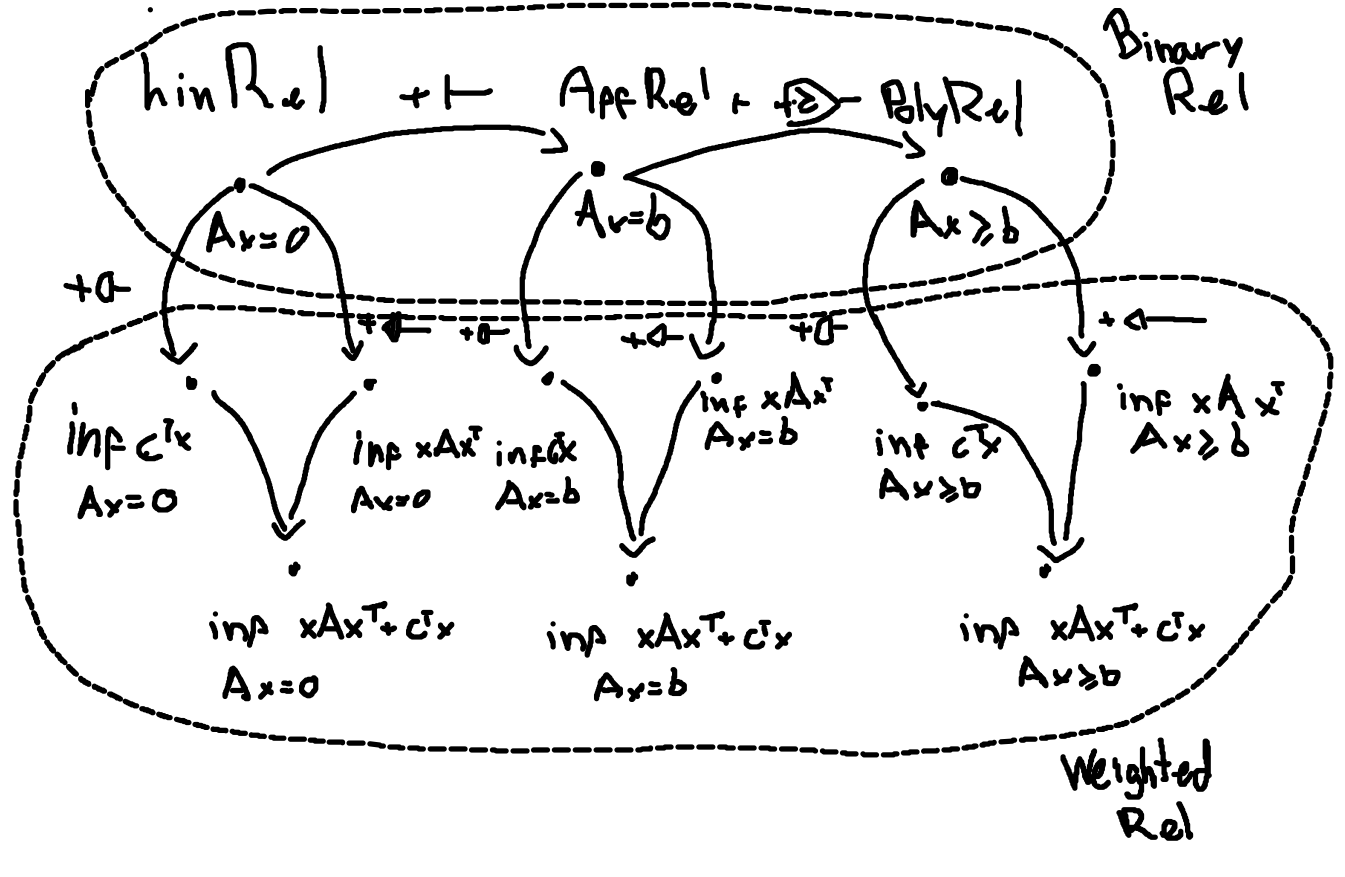
\includegraphics[width=1.0\linewidth]{../images/Overview.png}
    \caption{This image represents the category of subcategories of Rel; we circle two classes of subcategories,
    namely those that are contained in the Binary Relations categories and those embedded in the Weighted Relations category.
    Observe how morphisms between objects (classes of relations) are the addition of a single generator (along with some axioms),
    and that there are particular generators which are essentially binary relations (those that are horizontal) that
    keep objects in the subclass of binary relations, but there are others (the vertical morphisms),
    that resemble an output or measurement, that lift the relations to those on the Weighted Relations class.
    }
    \label{img:general_view}
\end{figure}

This expressivity becomes especially apparent when analyzed through
the language of string diagrams \cite{joyal1991geometry, selinger2010survey, piedeleu2023introductionstringdiagramscomputer}.
Originating as a rigorous graphical language for
monoidal categories, string diagrams provide an intuitive yet mathematically
precise syntax in which the sequential and parallel composition of morphisms
correspond directly to vertical and horizontal juxtaposition of diagrams
\cite{joyal1991geometry, maclane1998categories}. Building on this foundation,
a rich family of \emph{diagrammatic} or \emph{graphical calculi} has emerged,
offering complete axiomatisations of various algebraic structures purely through
equational diagram rewriting \cite{selinger2010survey, bonchi2017interacting}.
These calculi have proved remarkably versatile, finding applications across a
wide range of fields: in \emph{quantum computing} \cite{coecke2011interacting};
\emph{electronics} \cite{baez2018compositional}; \emph{linear algebra} \cite{bonchi2017interacting,
bonchi2019affine, defreitas2025generalizinginvertiblematrixtheorem};
and in \emph{optimisation and probability} \cite{stein2024gqa,stein2025compositional,
bonchi2021polyhedral}. Throughout this work
we explore how, step by step, one can enrich the already known theories for linear
\cite{bonchi2017interacting} algebra by adding one new generator at a time, along with a particular
set of axioms, and derive even richer structures for convex problems \cite{stein2024compositional}.

A first instance of this mechanism is the Graphical Quadratic Algebra (\textbf{GQA}) \cite{stein2024gqa},
where the addition of a single ``measurement'' generator expands the expressivity of the previous theories
by acting as a sort of measurement device along the diagram, lifting diagrams from the class of binary relations
to the broader class of weighted relations. From the optimization perspective, this is what plays the role of
the objective function in an optimization problem. We do not develop the quadratic branch here, but it serves
as the conceptual template for the cost generator at the heart of our contribution.

The polyhedral branch is the one our work builds on directly. Extending the Symmetric Monoidal Theory of
Graphical Affine Algebra (\textbf{GAA}) \cite{bonchi2019affine} with an inequality generator $-\ge -$ yields
Graphical Polyhedral Algebra (\textbf{GPA}) \cite{bonchi2021polyhedral}. Geometrically,
this allows the algebra to go beyond affine spaces and start representing polyhedral figures as linear inequality constraints in optimization,
\[
 \{| x \in P\} =
 \begin{cases}
     0 \quad \text{if} \;Ax +b\ge 0 \\
     +\infty \quad \text{otherwise.}
 \end{cases}
\]
Inspired by these observations, we make our central contribution: the introduction of a graphical
algebra for parametric linear programming. In this
setting, a linear program is no longer viewed only as
a numerical problem to be solved, but as a morphism that
can be composed with other optimization blocks.
This gives a symbolic language in which the elimination of internal variables
corresponds directly to categorical composition, allowing optimization problems
to be manipulated diagrammatically before computation.

In particular, every piecewise affine convex function can be represented as the value function of a linear program \cite{rockafellar1970convex}, which means the Graphical Linear Programming (\textbf{GLP}) theory provides a syntax for a broad class of nonsmooth convex models that appear in optimization, control, economics, and machine learning~\cite{boyd2004convex}. In Section~\ref{sec:glp} we show the diagrammatic equivalence of these two classes of objects and how diagrammatically they are not only denotationally equivalent but in fact instances of the same normal form. Thus, our diagrammatic syntax blurs the distinction between expressing LP programs as optimization problems and as piecewise convex functions, deriving a canonical normal form.

More broadly, this work suggests that graphical methods can play for optimization the same role that graphical linear algebra plays for matrices: providing normal forms, symbolic rewriting rules, and completeness results within a rigorous categorical setting. This opens the possibility of using diagrammatic reasoning not only for proofs, but also for designing compositional optimization systems and formal symbolic calculi for convex programming.

\paragraph{Overview}
Section~\ref{sec:bg} introduces the algebraic and categorical playground on which the
rest of the work is built: the initial notions of quantales and relations, the Extended-Lawvere
quantale of costs, the language of symmetric monoidal theories, and the prior graphical theories
$\mathbf{GLA}$, $\mathbf{GAA}$ and $\mathbf{GPA}$ on which our contribution rests.
Section~\ref{sec:sem} introduces, for the first time, the categorical semantics of parametric linear
programs, establishing the equivalence between piecewise affine convex functions, polyhedral
functions and parametric linear programs, and packaging them as the categories $\mathbf{LPRel}$ and
$\mathbf{PolyFun}$. Section~\ref{sec:glp} defines the symmetric monoidal theory $\mathbf{GLP}$,
its normal form, and the epigraph form. Section~\ref{sec:complete} proves soundness, definability
and completeness, establishing that $\mathbf{GLP}$ axiomatises the semantics.
This work represents a first step toward a complete diagrammatic calculus for convex optimization.

\section{Background}\label{sec:bg}

In this section we present the theory responsible for formalizing the field of diagrammatical
algebras and the necessary constructions to do so.
Also, a brief introduction to previous works will be presented in order to provide
the necessary notions and results that will be used later.

This section is outlined as follows: firstly, we present the background theory of quantales and
how they provide a suitable theory and algebraic form to express relations in a general sense.
Secondly,we offer a brief introduction of the categorical field of formal semmantics and what are
monoidal theories and how tey are used to build the syntax of diagrammatical calculis. Lastly, we
present the existing different theories and their semmantics where our work is built on, namely that of
Graphical Linear Algebra~\cite{paixao2022highlevel, bonchi2017interacting}, Graphical Affine Algebra~\cite{bonchi2019affine} and Graphical Polyhedral Algebra~\cite{bonchi2021polyhedral,bonchi2021.9farkas}.

\subsection{Ground definitions for relations}

While much of mathematical theory is built on functional thinking,
we argue that most of mathematics actually has a relational nature.
Category theory is the natural language for this purpose. It is precisely built on top of this notion,
in which everything one needs to know about an object is determined by its morphisms.

To begin we define the most basic kind of relation:

\begin{definition}[Binary Relations]
Let $X$ and $Y$ be sets. A \emph{binary relation} $R$ from $X$ to $Y$ is a subset
\[
R \subseteq X \times Y.
\]
Equivalently, it can be identified with its characteristic function
\[
\chi_R : X \times Y \to \{0,+\infty\},
\]
defined by
\[
\chi_R(x,y) =
\begin{cases}
0  \text{ if } (x,y) \in R,\\
+\infty \quad \text{otherwise}.
\end{cases}
\]
\end{definition}

A binary relation specifies whether $x$ is related to $y$.
Observe that one can think of a relation in two different ways that will prove useful later:
first, as a set of pairs, where every relation is just a pair $(x,y) \in R$,
or as a map that has $x,y$ as inputs and outputs $0$ if they are related, and $+\infty$ if they are not
(the choice of $\infty$ is arbitrary and will be justified later; normal choices here are actually $\{\text{true},\text{false}\}$ or $\{0,1\}$).

This is a general construct, as the sets $X$ and $Y$ can be anything.
We can, for instance, ask for further structures on such sets and obtain different kinds of relations.
\begin{definition}[Linear/Affine Relations]
Let $X$ and $Y$ be vector spaces. A \emph{linear relation} from $X$ to $Y$ is a linear subspace
\[
R \subseteq X \times Y.
\]
An \emph{affine relation} is an affine subspace of $X \times Y$.
Equivalently, a linear relation can be described as the graph of a possibly multivalued linear operator, i.e.,
\[
R(x) := \{ y \in Y \mid (x,y) \in R \}.
\]
\end{definition}

Thus, a linear/affine relation is a binary relation where the set $R$ is a subspace.
Notice, however, that we have been restricting the relations between $x$ and $y$ to be a case of ``they are, or they are not related''. In fact, we might be interested in adding degrees to such a relation, so that we could say that $x$ and $y$ are ``more'' or ``less'' related. This leads us to the well-known notion of weighted relations \cite{lawvere1973metric}.

\begin{definition}[Weighted Relations]
Let $X$ and $Y$ be any two sets and let $\extendR^+:= [0, +\infty]$.
A \emph{weighted relation} from $X$ to $Y$ is a set
\[
R \subseteq X \times Y \times \extendR^+
\]
such that for every $(x,y) \in X \times Y$ there exists \emph{exactly one}
$r \in \extendR^+$ satisfying $(x,y,r) \in R$.
Equivalently, we may define the characteristic function
$\chi_R : X \times Y \to \extendR^+$
by $\chi_R(x,y) = r$ if and only if $(x,y,r) \in R$.
\end{definition}

In fact, one could choose any other set instead of $\extendR^+$ to be the codomain of the characteristic function, as long as it satisfies some properties. The whole structure of a relation is further generalized by the notion of a quantale~\cite{rosenthal1990quantales}.
\begin{definition}[Quantale]
A \emph{quantale} is a structure $(Q,\leq,\otimes,e)$ such that:
\begin{itemize}
    \item $(Q,\leq)$ is a complete lattice, i.e., every subset $A \subseteq Q$ admits a join $\bigvee A$ and a meet $\bigwedge A$;
    \item $(Q,\otimes,e)$ is a monoid;
    \item Multiplication distributes over arbitrary join in each variable:
    \[
    a \otimes \Big( \bigvee_{i \in I} b_i \Big)
    =
    \bigvee_{i \in I} (a \otimes b_i),
    \qquad
    \Big( \bigvee_{i \in I} a_i \Big) \otimes b
    =
    \bigvee_{i \in I} (a_i \otimes b)
    \]
    for all families $\{a_i\}_{i\in I}, \{b_i\}_{i\in I} \subseteq Q$.
\end{itemize}
If $\otimes$ is commutative, the quantale is called \emph{commutative}.
If $e = \top$ (the top element of the lattice), it is called \emph{integral}.
\end{definition}

Given a quantale $Q$, we can define the notion of $Q$-valued relation \cite{coecke2018generalizedrelations}.

\begin{definition}[Generalized Relations]
A \emph{generalized relation} (or $Q$-valued relation) from $X$ to $Y$, where $Q$ is a quantale, is a set
$R \subseteq X \times Y \times Q$
such that for every $(x,y) \in X \times Y$ there exists \emph{exactly one}
$q \in Q$ satisfying $(x,y,q) \in R$.
Its characteristic function is $\chi_R: X \times Y \to Q$
defined by $\chi_R(x,y) = q$ if and only if $(x,y,q) \in R$.
\end{definition}

The notion of a $Q$-valued relation recovers familiar concepts for particular choices of quantale. For the (Boolean) truth quantale $Q = \{0,1\}$ with $\otimes = \land$ and $e = 1$, $Q$-valued relations coincide with classical binary relations. For the Lawvere quantale $Q = \extendR^+$ ordered by the reverse of the usual order, with $\otimes = +$ and $e = 0$, a $Q$-valued relation is precisely a weighted relation assigning a (possibly infinite) cost to each pair. Hence generalized relations unify ordinary binary relations and weighted relations as special cases corresponding to particular quantales.

Within this framework, we propose an extension of the Lawvere Quantale and
weighted relations called the Extended-Lawvere Quantale and
the Cost/Reward Relations, respectively. To our knowledge, this definition does
not appear elsewhere in the literature.

\begin{definition}[Optimization/Extended Lawvere Quantale]
Let $\overline{\mathbb{R}} := \mathbb{R} \cup \{-\infty,+\infty\}$.
The \emph{optimization quantale} is the structure $(\overline{\mathbb{R}},\geq,\otimes,e)$
defined as follows:
\begin{itemize}
    \item The order $\geq$ is the usual order on the extended real line.
    With this order, arbitrary joins are given by the usual infima: $\bigvee A = \inf A$.
    \item The monoidal product is addition $a \otimes b := a + b$,
    where addition is extended in the usual way
    (with $a + (+\infty) = +\infty$ and $a + (-\infty) = -\infty$ whenever defined).
    \item The unit element is $e := 0$.
\end{itemize}
With these operations, $(\overline{\mathbb{R}},\geq,+,0)$
is a commutative quantale. Joins are ordinary infima,
and addition distributes over arbitrary joins.
\end{definition}

\begin{definition}[Optimization (Cost/Reward) Relations]
Let $X$ and $Y$ be sets.
An \emph{optimization relation} from $X$ to $Y$ is an
$\overline{\mathbb{R}}$-valued relation, i.e., a function
$R : X \times Y \to \overline{\mathbb{R}}$.
The value $R(x,y)$ is interpreted as the objective value
(cost or reward) associated to the pair $(x,y)$,
with $+\infty$ and $-\infty$ representing extremal infeasibility
or unboundedness.
\end{definition}

Observe how this is essentially the weighted relations extended
along the negative values. The importance of it is that we want
to be able to express optimization problems that might be infeasible
($+\infty$) or unbounded ($-\infty$), so we need to add both
the top and bottom element.

All of this admits a suitable and natural categorical construction.
Specifically, from any quantale $Q$ one can not only define $Q$-relations,
but also construct an entire category of them.
This category is the natural setting for discussing the
central concept of this framework: the composition of relations.
The following proposition shows how to build such a category and establishes
that it carries a very important monoidal structure;
particularly, it is a compact closed
symmetric monoidal category~\cite{maclane1998categories}.

\begin{proposition}[Category $\mathbf{Rel}(Q)$]
For a quantale $Q$, the $Q$-relations form a category $\mathbf{Rel}(Q)$ with composition and identities
\[
(S\circ R) (a,c) = \bigvee_b R(a,b) \otimes S(b,c), \quad 1_A(a,b) = \bigvee \{e \mid a=b\}.
\]
If $Q$ is a commutative quantale, then $\mathbf{Rel}(Q)$ carries a symmetric monoidal structure, with the categorical monoidal product $\bigotimes_{\mathcal{C}}$ on objects given by the Cartesian product of sets and the action on relations given for $R:A \to C$ and $S:B\to D$ by
\[
(R\otimes_{\mathcal{C}} S)(a,b,c,d) = R(a,c) \otimes S(b,d).
\]
The singleton set is the monoidal unit, and the category is compact closed w.r.t.\ the monoidal structure.
\end{proposition}

\begin{proof}
We verify the categorical structure.

\medskip
\noindent
\textbf{(1) Well-defined composition.}
Let $R:A \to B$ and $S:B \to C$ be $Q$-relations.
For each $(a,c) \in A \times C$, the set
$\{ R(a,b)\otimes S(b,c) \mid b \in B \} \subseteq Q$
admits a supremum since $Q$ is a complete lattice.
Hence $(S\circ R)(a,c)$ is well-defined as an element of $Q$.

\medskip
\noindent
\textbf{(2) Associativity.}
Let $R:A\to B$, $S:B\to C$, and $T:C\to D$.
For $a\in A$, $d\in D$,
\[
((T\circ S)\circ R)(a,d)
=
\bigvee_{c}
\Big(
\bigvee_{b} R(a,b)\otimes S(b,c)
\Big)
\otimes T(c,d).
\]
Since $\otimes$ distributes over arbitrary suprema,
$= \bigvee_{b,c} R(a,b)\otimes S(b,c)\otimes T(c,d)$.
Similarly,
\[
(T\circ (S\circ R))(a,d)
=
\bigvee_{b}
R(a,b)\otimes
\Big(
\bigvee_{c} S(b,c)\otimes T(c,d)
\Big)
=
\bigvee_{b,c}
R(a,b)\otimes S(b,c)\otimes T(c,d).
\]
Thus composition is associative.

\medskip
\noindent
\textbf{(3) Identities.}
For each set $A$, define
\[
1_A(a,b)
=
\begin{cases}
e & \text{if } a=b,\\
\bot & \text{otherwise},
\end{cases}
\]
where $\bot = \bigvee \varnothing$ is the bottom element of $Q$.
Then for $R:A\to B$,
$(R\circ 1_A)(a,b) = \bigvee_{a'} 1_A(a,a')\otimes R(a',b)$.
All terms vanish except when $a'=a$, so this equals $e \otimes R(a,b) = R(a,b)$.
Similarly, $1_B\circ R = R$. Hence identities exist.

\medskip
\noindent
\textbf{(4) Monoidal structure (commutative case).}
Assume $Q$ is commutative.
Define the tensor on objects by Cartesian product $A\otimes_{\mathcal{C}} B := A\times B$.
For relations $R:A\to C$ and $S:B\to D$, define
$(R\otimes_{\mathcal{C}} S)((a,b),(c,d)) = R(a,c)\otimes S(b,d)$.
Functoriality follows from associativity and commutativity of $\otimes$:
$(S_1\otimes S_2)\circ (R_1\otimes R_2) = (S_1\circ R_1)\otimes (S_2\circ R_2)$.
The singleton set $1$ is a unit since $A\times 1 \cong A$.
Symmetry is induced by the swap map.

\medskip
\noindent
\textbf{(5) Compact closure.}
For each set $A$, define unit and counit relations
$\eta : 1 \to A\times A$ and $\epsilon : A\times A \to 1$
by $\eta(*,(a,a')) = e$ if $a=a'$ ($\bot$ otherwise) and
$\epsilon((a,a'),*) = e$ if $a=a'$ ($\bot$ otherwise).
A direct computation using the definition of composition shows that the
triangle identities hold:
\[
(1_A\otimes \epsilon)\circ (\eta\otimes 1_A) = 1_A,
\qquad
(\epsilon\otimes 1_A)\circ (1_A\otimes \eta) = 1_A.
\]
Thus every object is self-dual, and $\mathbf{Rel}(Q)$ is compact closed.
\end{proof}

A curious fact about relations is that they actually encode the notion of matrices and matrix multiplication. A $Q$-valued relation $R : X \times Y \to Q$ is nothing but a \emph{$Q$-valued matrix} indexed by $X \times Y$, and composition of $Q$-valued relations corresponds precisely to matrix multiplication in $Q$, where ordinary addition is replaced by the join $\bigvee$ and ordinary multiplication by the monoidal product $\otimes$. The two axioms of a quantale --- that $\otimes$ distributes over arbitrary joins --- are precisely what guarantees that this multiplication is associative and well-defined. This serves as motivation for what will later become the diagrammatical theory of linear algebra.

The resulting categories are symmetric monoidal, and it is precisely this monoidal backbone that will support the algebraic structure we aim to build. A key piece of that structure is a \emph{Frobenius monoid} on each object: a monoid $(\mu, \eta)$ and a comonoid $(\delta, \varepsilon)$ on the same object, satisfying the Frobenius law
\[
  (\mathrm{id} \otimes \mu) \circ (\delta \otimes \mathrm{id})
  \;=\;
  \delta \circ \mu
  \;=\;
  (\mu \otimes \mathrm{id}) \circ (\mathrm{id} \otimes \delta).
\]
A symmetric monoidal category in which every object carries such a structure, compatibly with the tensor product, is called a \emph{hypergraph category} \cite{fong2019hypergraph}. Hypergraph categories are related to, but strictly more general than, compact closed categories \cite{selinger2010survey}, and it is the more general notion that we adopt as our ambient framework.

\begin{remark}
    If $Q$ is commutative, then $\mathbf{Rel}(Q)$ is a hypergraph category~\cite{fong2019hypergraph} and admits a commutative Frobenius structure on every object. Diagrammatically, we denote the additive and co-additive structure as
    \begin{figure}[H]
        \centering
        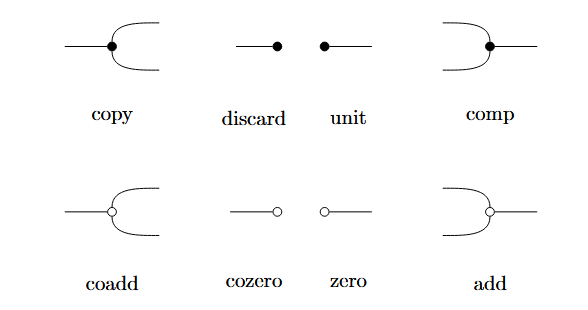
\includegraphics[width=1\linewidth]{../images/froberniusDiagram.png}
        \caption{Frobenius additive (black) and co-additive (white) structure.}
    \end{figure}
    subject to the Frobenius Law (both colors)
   \begin{figure}[H]
        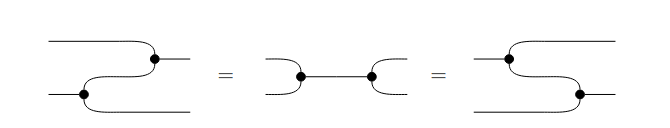
\includegraphics[width=1\linewidth]{../images/FroberniusLaw.png}
    \end{figure}
\end{remark}

\subsection{Syntax: Symmetric Monoidal Theories}

These constructions provide exactly the semantic foundation for the algebra we aim to build. In the same way that semantics is understood in linguistics and programming language theory \cite{winskel1993formal}, the semantics of a formal system assigns meaning to its expressions. More precisely, while syntax consists of the tokens and rules for forming and combining expressions, semantics is the interpretation assigned to each such expression --- in our case, an optimization problem living in $\mathbf{Rel}(Q)$.

As outlined in the introduction, the central goal of this work is to show that optimization emerges naturally from algebraic and categorical structure.
The key mechanism enabling this is the infimal composition present in the definition of the Cost/Reward category: composing two relations automatically performs variable elimination, which is precisely the fundamental operation underlying optimization.

To make this precise, we need both a semantics --- provided by the categorical framework developed above --- and a syntax: a rigorous, compositional language for expressing optimization problems symbolically.
The map between those is a structure-preserving map, a functor, from the syntactic layer into the semantic one.
The syntactic layer will be formalized as a Symmetric Monoidal Theory (SMT) \cite{bonchi2017interacting}, a presentation of a category by generators and equations, whose terms respect the compositional structure of a symmetric monoidal category.

\begin{definition}[Symmetric Monoidal Theory]
    An SMT is a pair $(\Sigma,E)$ such that $\Sigma$ is a signature of operators $o$ with arity $m$ and coarity $n$.
    $\Sigma$-terms are defined inductively as the smallest collection of
typed expressions $t : m \to n$ closed under: generators $o \in \Sigma$;
identities $\mathrm{id}_n : n \to n$; composition $a;b : m\to k$ for $a:m\to n$, $b:n\to k$;
tensor product $a \otimes b : m_1+m_2 \to n_1+n_2$ for $a:m_1\to n_1$, $b:m_2\to n_2$;
and symmetries $\sigma_{m,n} : m+n \to n+m$.
And $E$ is a set of equations over the $\Sigma$-terms.
\end{definition}

Often, we will think of elements $o:m\to n \in \Sigma$ as generators and represent them as string diagrams, the $\Sigma$-terms being the results of composing those generators horizontally and vertically inductively, and the set $E$ as a collection of axiomatic equations over these string diagrams. The categorical counterpart of these terms is the free category generated by the SMT.

\begin{definition}[The Free category of an SMT]
    The $\text{FreeP}_{(\Sigma,E)}$ is the category freely generated by $(\Sigma,E)$ where the objects are natural numbers, morphisms are $\Sigma$-terms quotiented by $E$, with composition and tensor product inherited from the symmetric monoidal structure. $\text{FreeP}_{(\Sigma,E)}$ is in fact a PROP\footnote{For the definition of a PROP see~\cite{maclane1998categories}.}.
\end{definition}

The $\text{FreeP}_{(\Sigma,E)}$, also denoted $P\Sigma_{/E}$,\footnote{During the work we will use $\text{FreeP}_{S}$ and $S$, for whatever syntax $S$ may be, interchangeably.}
will be our \textbf{syntax} responsible for expressing our underlying semantics.
For it to be considered a ``useful'' syntax we expect that it satisfies some properties, particularly we want it to be complete, sound and expressive. Without those, our algebra would be empty, since we would have no assurance that it actually says anything meaningful about what we desire to say.

\begin{definition}\label{def:definability}
    We will say that an SMT axiomatizes or represents a specific category, usually called the semantic category, when the following diagram commutes:
    \begin{figure}[H]
        \centering
        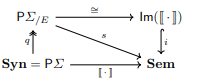
\includegraphics[width=0.35\linewidth]{../images/Definibilty.png}
    \end{figure}
    where $P\Sigma$ is the category where objects are natural numbers and morphisms are $\Sigma$-terms from $n \to m$; $P\Sigma_{/E} = \text{FreeP}_{(\Sigma,E)}$ is the $P\Sigma$ category with the morphisms quotiented by $E$ and there is then a PROP morphism $q : P\Sigma \to P\Sigma_{/E}$ witnessing this quotient; $\textbf{Sem}$ is our semantic category (the Cost/Reward relations for example); and $s$ is a full and faithful PROP morphism. Another way to say the same is to demand two things out of the SMT:
\begin{itemize}
    \item Soundness: $P\Sigma_{/E}$ is sound if $c \overset{E}= d$\footnote{$\overset{E}=$ means that this equality is provable by the equations in $E$.} implies $[c] = [d]$.
    \item Completeness: $P\Sigma_{/E}$ is complete if $[c] = [d]$ implies $c \overset{E}= d$.
    \item Expressivity: $P\Sigma_{/E}$ is expressive if for every morphism $c$ in \textbf{Sem} there exists $d \in P\Sigma_{/E}$ such that $[d] = c$.
\end{itemize}
\end{definition}

Those three properties capture the idea that everything we can prove in the syntax holds in the semantics (soundness), everything that holds in the semantics is provable in the syntax (completeness), and that every morphism in the semantics has a syntactic representative (expressivity). Moreover, these properties denote equivalent characteristics about the interpretation map, both categorically and functionally, as depicted in Table~\ref{tab:equivalences}.

\begin{table}[h!]
\centering
\caption{Equivalence of properties for the interpretation map
         $[\![{-}]\!] : P\Sigma_{/E} \to \mathbf{Sem}$}
\label{tab:equivalences}
\begin{tabular}{
  m{3.2cm}
  m{3.2cm}
  m{4.5cm}
}
\toprule
\textbf{Set theory} &
\textbf{Category theory} &
\textbf{Logic (SMT)} \\
\midrule
Total &
Functor &
Soundness: $c \overset{E}{=} d \;\Rightarrow\; [\![c]\!] = [\![d]\!]$ \\[6pt]
Deterministic &
Well-defined map &
(Functionality of the interpretation) \\[6pt]
Injective &
Faithful &
Completeness: $[\![c]\!] = [\![d]\!] \;\Rightarrow\; c \overset{E}{=} d$ \\[6pt]
Surjective &
Full &
Expressivity: $\forall\, f \in \mathbf{Sem},\; \exists\, d \in P\Sigma_{/E} \text{ s.t. } [\![d]\!] = f$ \\
\bottomrule
\end{tabular}
\end{table}

\subsection{Previous algebras}

We now introduce the foundational theories for Graphical Algebra that serve as a foundation for the following sections, namely Graphical Linear Algebra~\cite{paixao2022highlevel, bonchi2017interacting}, Graphical Affine Algebra~\cite{bonchi2019affine}, and Graphical Polyhedral Algebra~\cite{bonchi2021polyhedral}. Each of them being a extension of the previous one, meaning that there's a structure preserve inclusion functor $\mathbf{GLA} \hookrightarrow \mathbf{GAA} \hookrightarrow \mathbf{GLP}$.

\begin{definition}
    We will call $\textbf{GLA}$ the presentation of the Graphical Linear Algebra SMT, in the same manner, $\textbf{GAA}$ the SMT of Graphical Affine Algebra and \textbf{GPA} the SMT of Graphical Polyhedral Algebra. Below we show, separatedly, the set of generators(the signature $\Sigma$) of each one of them.

    \begin{center}
    \begin{tikzpicture}[
        boxnode/.style={rounded rectangle, fill=white, draw=black, inner sep=4pt, anchor=center},
        boxlabel/.style={anchor=south west, font=\bfseries}]

        % ---- GLA: the linear-algebra generators ----
        \pic (a1) at (0,0)    {copy};
        \pic (a2) at (1.8,0)  {cocopy};
        \pic (a3) at (3.6,0)  {discard};
        \pic (a4) at (5.4,0)  {codiscard};
        \pic (a5) at (0,-1.5)   {multiplication};
        \pic (a6) at (1.8,-1.5) {comultiplication};
        \pic (a7) at (3.6,-1.5) {zero};
        \pic (a8) at (5.4,-1.5) {cozero};
        \pic [val=k] (a9) at (3.2,-2.7) {scalar};
        \draw[rounded corners, thick] (-0.9,-3.5) rectangle (6.3,0.9);
        \node[boxlabel] at (-0.9,1.0) {$\mathbf{GLA}$};

        % ---- GAA: adds the affine (constant) generator ----
        \pic (b1) at (0,-4.5) {affine};
        \draw[rounded corners, thick] (-0.9,-5.0) rectangle (1.3,-4.0);
        \node[boxlabel] at (-0.9,-3.98) {$\mathbf{GAA} = \mathbf{GLA} \;+$};

        % ---- GPA: adds the inequality generator ----
        \pic (c1) at (0,-6.1) {ge};
        \draw[rounded corners, thick] (-0.9,-6.6) rectangle (1.3,-5.6);
        \node[boxlabel] at (-0.9,-5.58) {$\mathbf{GPA} = \mathbf{GAA} \;+$};
    \end{tikzpicture}
    \end{center}

    and the axioms, previously called the set $E$ of equations for the SMT.

    \tikzset{
      axpic/.style={baseline=(current bounding box.center), x=0.6cm, y=0.52cm, line cap=round},
      boxnode/.style={rounded rectangle, fill=white, draw=black, inner sep=2pt, anchor=center}
    }

    \medskip
    \noindent\fbox{\begin{minipage}{0.97\linewidth}
    \begin{center}\textbf{$\mathbf{GLA}$ axioms}\quad{\footnotesize\cite{paixao2022highlevel,bonchi2017interacting}}\end{center}

    \textit{White commutative monoid (addition $\oplus$, unit $\circ$).}
    \begin{center}\begin{tabular}{r@{\quad}c@{\;$=$\;}c}
    (assoc) &
    \begin{tikzpicture}[axpic]
      \pic (m1) at (0,0.9) {multiplication};
      \pic (m2) at (1.7,0) {multiplication};
      \draw (m1-out-0) -- (m2-in-0);
    \end{tikzpicture}
    &
    \begin{tikzpicture}[axpic]
      \pic (m1) at (0,-0.9) {multiplication};
      \pic (m2) at (1.7,0) {multiplication};
      \draw (m1-out-0) -- (m2-in-1);
    \end{tikzpicture}
    \\[3mm]
    (comm) &
    \begin{tikzpicture}[axpic]
      \pic (m) at (1,0) {multiplication};
      \draw (-0.6,0.5) to (m-in-1);
      \draw (-0.6,-0.5) to (m-in-0);
    \end{tikzpicture}
    &
    \begin{tikzpicture}[axpic]
      \pic (m) at (0,0) {multiplication};
    \end{tikzpicture}
    \\[3mm]
    (unit) &
    \begin{tikzpicture}[axpic]
      \pic (z) at (-0.2,0.8) {zero};
      \pic (m) at (1,0) {multiplication};
      \draw (z-out-0) -- (m-in-0);
    \end{tikzpicture}
    &
    \begin{tikzpicture}[axpic]\pic (i) at (0,0) {identity};\end{tikzpicture}
    \end{tabular}\end{center}

    \textit{Black cocommutative comonoid (copy, counit $\bullet$).}
    \begin{center}\begin{tabular}{r@{\quad}c@{\;$=$\;}c}
    (coassoc) &
    \begin{tikzpicture}[axpic]
      \pic (c1) at (0,0.9) {copy};
      \pic (c2) at (1.7,0) {copy};
      \draw (c1-out-1) -- (c2-in-0);
    \end{tikzpicture}
    &
    \begin{tikzpicture}[axpic]
      \pic (c1) at (0,-0.9) {copy};
      \pic (c2) at (1.7,0) {copy};
      \draw (c1-out-0) -- (c2-in-0);
    \end{tikzpicture}
    \\[3mm]
    (cocomm) &
    \begin{tikzpicture}[axpic]
      \pic (c) at (0,0) {copy};
      \draw (c-out-0) to (1.6,-0.5);
      \draw (c-out-1) to (1.6,0.5);
    \end{tikzpicture}
    &
    \begin{tikzpicture}[axpic]
      \pic (c) at (0,0) {copy};
    \end{tikzpicture}
    \\[3mm]
    (counit) &
    \begin{tikzpicture}[axpic]
      \pic (c) at (0,0) {copy};
      \pic (d) at (1.4,0.5) {discard};
      \draw (c-out-0) -- (d-in-0);
    \end{tikzpicture}
    &
    \begin{tikzpicture}[axpic]\pic (i) at (0,0) {identity};\end{tikzpicture}
    \end{tabular}\end{center}

    \textit{Bialgebra / Hopf (white over black).}
    \begin{center}\begin{tabular}{r@{\quad}c@{\;$=$\;}c}
    (B1) &
    \begin{tikzpicture}[axpic]
      \pic (a) at (0,0) {multiplication};
      \pic (c) at (1.6,0) {copy};
      \draw (a-out-0) -- (c-in-0);
    \end{tikzpicture}
    &
    \begin{tikzpicture}[axpic]
      \pic (c1) at (0,1.7) {copy};
      \pic (c2) at (0,-1.7) {copy};
      \pic (a1) at (2.2,1.7) {multiplication};
      \pic (a2) at (2.2,-1.7) {multiplication};
      \draw (c1-out-0) -- (a1-in-0);
      \draw (c2-out-1) -- (a2-in-1);
      \draw (c1-out-1) to (a2-in-0);
      \draw (c2-out-0) to (a1-in-1);
    \end{tikzpicture}
    \\[3mm]
    (B2) &
    \begin{tikzpicture}[axpic]
      \pic (a) at (0,0) {multiplication};
      \pic (d) at (1.4,0) {discard};
      \draw (a-out-0) -- (d-in-0);
    \end{tikzpicture}
    &
    \begin{tikzpicture}[axpic]
      \pic (d1) at (0,0.7) {discard};
      \pic (d2) at (0,-0.7) {discard};
    \end{tikzpicture}
    \\[3mm]
    (B3) &
    \begin{tikzpicture}[axpic]
      \pic (z) at (-0.6,0) {zero};
      \pic (c) at (0.8,0) {copy};
      \draw (z-out-0) -- (c-in-0);
    \end{tikzpicture}
    &
    \begin{tikzpicture}[axpic]
      \pic (z1) at (0,0.7) {zero};
      \pic (z2) at (0,-0.7) {zero};
    \end{tikzpicture}
    \\[3mm]
    (B4, unit) &
    \begin{tikzpicture}[axpic]
      \pic (z) at (-0.6,0) {zero};
      \pic (d) at (0.8,0) {discard};
      \draw (z-out-0) -- (d-in-0);
    \end{tikzpicture}
    &
    \begin{tikzpicture}[axpic]\path(-0.6,-0.6) rectangle (0.6,0.6);\node{};\end{tikzpicture}
    \end{tabular}\end{center}

    \textit{Frobenius and special law (copy structure; the addition structure is dual).}
    \begin{center}\begin{tabular}{r@{\quad}c@{\;$=$\;}c}
    (Frob) &
    \begin{tikzpicture}[axpic]
      \pic (c) at (0,0.7) {copy};
      \pic (m) at (1.7,-0.6) {cocopy};
      \draw (c-out-1) -- (m-in-0);
    \end{tikzpicture}
    &
    \begin{tikzpicture}[axpic]
      \pic (m) at (0,0) {cocopy};
      \pic (c) at (1.7,0) {copy};
      \draw (m-out-0) -- (c-in-0);
    \end{tikzpicture}
    \\[3mm]
    (special) &
    \begin{tikzpicture}[axpic]
      \pic (c) at (0,0) {copy};
      \pic (m) at (1.5,0) {cocopy};
      \draw (c-out-0) -- (m-in-0);
      \draw (c-out-1) -- (m-in-1);
    \end{tikzpicture}
    &
    \begin{tikzpicture}[axpic]\pic (i) at (0,0) {identity};\end{tikzpicture}
    \end{tabular}\end{center}

    \textit{Scalars and antipode ($\text{-}1$).}
    \begin{center}\begin{tabular}{r@{\quad}c@{\;$=$\;}c}
    (s.\,add) &
    \begin{tikzpicture}[axpic]
      \pic (c) at (0,0) {copy};
      \pic [val=k] (sk) at (1.6,0.9) {scalar};
      \pic [val=l] (sl) at (1.6,-0.9) {scalar};
      \pic (a) at (3.2,0) {multiplication};
      \draw (c-out-0) -- (sk-in-0);
      \draw (c-out-1) -- (sl-in-0);
      \draw (sk-out-0) -- (a-in-0);
      \draw (sl-out-0) -- (a-in-1);
    \end{tikzpicture}
    &
    \begin{tikzpicture}[axpic]\pic [val={k+l}] (s) at (0,0) {scalar};\end{tikzpicture}
    \\[3mm]
    (s.\,mult) &
    \begin{tikzpicture}[axpic]
      \pic [val=k] (sk) at (0,0) {scalar};
      \pic [val=l] (sl) at (1.6,0) {scalar};
      \draw (sk-out-0) -- (sl-in-0);
    \end{tikzpicture}
    &
    \begin{tikzpicture}[axpic]\pic [val={kl}] (s) at (0,0) {scalar};\end{tikzpicture}
    \\[3mm]
    (antipode) &
    \begin{tikzpicture}[axpic]
      \pic (c) at (0,0) {copy};
      \pic [val={\text{-}1}] (sm) at (1.6,-0.9) {scalar};
      \pic (a) at (3.2,0) {multiplication};
      \draw (c-out-0) to (a-in-0);
      \draw (c-out-1) -- (sm-in-0);
      \draw (sm-out-0) -- (a-in-1);
    \end{tikzpicture}
    &
    \begin{tikzpicture}[axpic]
      \pic (d) at (-0.6,0) {discard};
      \pic (z) at (0.8,0) {zero};
    \end{tikzpicture}
    \end{tabular}\end{center}
    \end{minipage}}

    \medskip
    \noindent\fbox{\begin{minipage}{0.97\linewidth}
    \begin{center}\textbf{$\mathbf{GAA}$ axioms (in addition to $\mathbf{GLA}$)}\quad{\footnotesize\cite{bonchi2019affine}}\end{center}
    The affine generator $\rtop$ (a point $0\to 1$, drawn as the empty box) is a comonoid homomorphism:
    \begin{center}\begin{tabular}{r@{\quad}c@{\;$=$\;}c}
    (aff.\,copy) &
    \begin{tikzpicture}[axpic]
      \pic (t) at (-0.6,0) {affine};
      \pic (c) at (0.8,0) {copy};
      \draw (t-out-0) -- (c-in-0);
    \end{tikzpicture}
    &
    \begin{tikzpicture}[axpic]
      \pic (t1) at (0,0.7) {affine};
      \pic (t2) at (0,-0.7) {affine};
    \end{tikzpicture}
    \\[3mm]
    (aff.\,del) &
    \begin{tikzpicture}[axpic]
      \pic (t) at (-0.6,0) {affine};
      \pic (d) at (0.8,0) {discard};
      \draw (t-out-0) -- (d-in-0);
    \end{tikzpicture}
    &
    \begin{tikzpicture}[axpic]\path(-0.6,-0.6) rectangle (0.6,0.6);\node{};\end{tikzpicture}
    \end{tabular}\end{center}
    \end{minipage}}

    \medskip
    \noindent\fbox{\begin{minipage}{0.97\linewidth}
    \begin{center}\textbf{$\mathbf{GPA}$ axioms (in addition to $\mathbf{GAA}$)}\quad{\footnotesize\cite{bonchi2021polyhedral}}\end{center}
    The order primitive $\ge$ is a preorder compatible with the linear structure
    (transitivity; monoid and comonoid morphism; $0\ge 0$):
    \begin{center}\begin{tabular}{r@{\quad}c@{\;$=$\;}c}
    (trans) &
    \begin{tikzpicture}[axpic]
      \pic (g1) at (0,0) {ge};
      \pic (g2) at (1.5,0) {ge};
      \draw (g1-out-0) -- (g2-in-0);
    \end{tikzpicture}
    &
    \begin{tikzpicture}[axpic]\pic (g) at (0,0) {ge};\end{tikzpicture}
    \\[3mm]
    (mono.\,$\oplus$) &
    \begin{tikzpicture}[axpic]
      \pic (a) at (0,0) {multiplication};
      \pic (g) at (1.5,0) {ge};
      \draw (a-out-0) -- (g-in-0);
    \end{tikzpicture}
    &
    \begin{tikzpicture}[axpic]
      \pic (g1) at (0,0.8) {ge};
      \pic (g2) at (0,-0.8) {ge};
      \pic (a) at (1.7,0) {multiplication};
      \draw (g1-out-0) -- (a-in-0);
      \draw (g2-out-0) -- (a-in-1);
    \end{tikzpicture}
    \\[3mm]
    (mono.\,copy) &
    \begin{tikzpicture}[axpic]
      \pic (c) at (0,0) {copy};
      \pic (g1) at (1.5,0.8) {ge};
      \pic (g2) at (1.5,-0.8) {ge};
      \draw (c-out-0) -- (g1-in-0);
      \draw (c-out-1) -- (g2-in-0);
    \end{tikzpicture}
    &
    \begin{tikzpicture}[axpic]
      \pic (g) at (0,0) {ge};
      \pic (c) at (1.5,0) {copy};
      \draw (g-out-0) -- (c-in-0);
    \end{tikzpicture}
    \\[3mm]
    (zero) &
    \begin{tikzpicture}[axpic]
      \pic (z) at (-0.6,0) {zero};
      \pic (g) at (0.8,0) {ge};
      \draw (z-out-0) -- (g-in-0);
    \end{tikzpicture}
    &
    \begin{tikzpicture}[axpic]\pic (z) at (0,0) {zero};\end{tikzpicture}
    \end{tabular}\end{center}
    Together with reflexivity, antisymmetry and positivity of scalars; see \cite{bonchi2021polyhedral,bonchi2021.9farkas}.
    \end{minipage}}

\end{definition}

\begin{definition}\label{def:arrows}
    We also denote with $\overrightarrow{(\cdot)}/\overleftarrow{(\cdot)}$ when we want to talk about the algebra generated without the Frobenius structure. For example $\overrightarrow{\textbf{GLA}}$ is the algebra generated by
    \begin{figure}[H]
        \centering
        
\includegraphics[width=.5\linewidth]{../images/RightAlgebra.png}
    \end{figure}
    without their symmetric
    \begin{figure}[H]
        \centering
        
\includegraphics[width=0.5\linewidth]{../images/LeftAlgebra.png}
    \end{figure}
    and the exactly opposite we denote as $\overleftarrow{\textbf{GLA}}$.
\end{definition}

The theory our contribution builds on directly is Graphical Polyhedral Algebra. Geometrically it goes beyond affine spaces, representing polyhedra as linear-inequality constraints. We begin by recalling the standard definitions.

\begin{definition}\label{polyform}
A set $P \subseteq \mathbb{R}^n$ is called a \emph{polyhedron} if there
exist $A \in \mathbb{R}^{m \times n}$ and $b \in \mathbb{R}^m$ such that
$P = \{x \in \mathbb{R}^n \mid Ax \ge b\}$.
\end{definition}

The corresponding semantic categories capture polyhedrals as morphisms, with relational composition playing the role of variable elimination.

\begin{definition}[The prop $\mathbf{PolyRel}$ of polyhedra]
Let $k$ be an ordered field. The prop $\mathbf{PolyRel}_k$ has objects natural numbers $n$, morphisms $n\to m$ the polyhedra $R \subseteq k^n \times k^m$ of the form
$R = \{ (x,y) \mid A (x,y)^\top + b \ge 0 \}$,
composition relational composition, and monoidal product addition on objects, Cartesian product on morphisms.
\end{definition}

The central computational primitive of the polyhedral theory is Fourier--Motzkin Elimination (FME)~\cite{schrijver1986theory, ziegler1995polytopes}, which projects a polyhedron onto a lower-dimensional space by eliminating one variable at a time. In $\mathbf{GPA}$ this is realized diagrammatically, after first establishing that the $\ge$ generator is transitive, reflexive and antisymmetric.

\begin{proposition}[Fourier--Motzkin Elimination]
The following diagrammatic procedure is equivalent to performing the FME algorithm:
\begin{figure}[H]
    \centering
    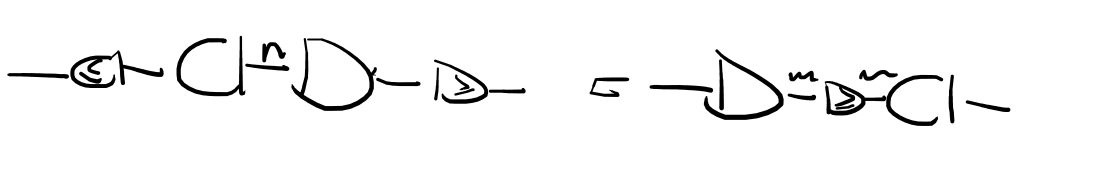
\includegraphics[width=1\linewidth]{../images/GPA/FMEDiag.png}
\end{figure}
\end{proposition}

Using FME, $\mathbf{GPA}$ admits a normal form, and applying the polar operator (the polyhedral analogue of Farkas duality, exchanging the $H$- and $V$-representations \cite{bonchi2021.9farkas}) yields a second, conic-hull normal form. These drive the presentation theorems below, whose proofs we recall from \cite{bonchi2021polyhedral}.

\begin{theorem}\label{thm:gpapresent}
    $\mathbf{PolyRel}$ is presented by $\mathrm{FreeP}_{\mathbf{GPA}}$.
\end{theorem}

This is the structural foundation on which our final contribution, $\mathbf{GLP}$, is built: there, these constraints are combined with a linear objective to form full parametric linear programs.

\section{The Semmantic of Linear Programs}\label{sec:sem}

Next, we introduce, for the first time, the categorical semmantics of Parametric linear
Programs (PLP). This section is self-contained. All results from the ordinary theory of linear programs, alongside with any categorical notion that are to be used here or later are to be defined and proved along it.

Results presented here, such as the existence of a standard form for PLP and certain
equivalences between their epigraph and value function will be of funamental importance
later when demonstrating the completeness of our algebra.

\subsection{Preliminary Results in Linear Programming}

We begin with several classical results that establish the tight
relationship between piecewise affine convex functions, polyhedral
functions, and parametric linear programs. These will serve as the
semantic foundation for the graphical algebra introduced in the following
section.

\begin{definition}[Piecewise Affine Convex Function]
A function $f : \mathbb{R}^n \to \mathbb{R}$ is called
\emph{piecewise affine convex} if there exist finitely many affine
functions $a_i^\top x + b_i$, $i = 1,\dots,k$, such that
\[
f(x) = \max_{i=1,\dots,k} \{ a_i^\top x + b_i \}.
\]
\end{definition}

\begin{definition}[Polyhedral Function]
A function $f : \mathbb{R}^n \to \mathbb{R} \cup \{+\infty\}$ is
\emph{polyhedral} if its epigraph
$\mathrm{epi}(f) := \{ (x,t) \mid t \ge f(x) \}$
is a polyhedron.
\end{definition}

\begin{definition}[RHS Parametric Linear Program]
A \emph{right-hand side parametric linear program} has value function
$v(b) := \inf_{x} \{ c^\top x \mid Ax \ge b \}$.
\end{definition}

The following two propositions establish that all three notions above
are equivalent descriptions of the same class of functions. This
equivalence is the semantic cornerstone of the section: it is what
allows us to treat polyhedral functions and parametric linear programs
as morphisms in the same category.

\begin{proposition}
A function is piecewise affine convex if and only if it is a polyhedral
function.
\end{proposition}

\begin{proof}
\textbf{($\Rightarrow$)} Let
$f(x) = \max_{i=1,\dots,k} (a_i^\top x + b_i)$.
Then
\[
\mathrm{epi}(f) = \bigcap_{i=1}^k \{ (x,t) \mid t \ge a_i^\top x + b_i \},
\]
which is an intersection of finitely many halfspaces, hence a polyhedron.

\medskip
\textbf{($\Leftarrow$)} If $f$ is polyhedral, its epigraph is a
polyhedron, so there exist finitely many affine inequalities
$t \ge a_i^\top x + b_i$ such that
$f(x) = \max_{i=1,\dots,k} (a_i^\top x + b_i)$.
Thus $f$ is piecewise affine and convex.
\end{proof}

\begin{proposition}
A function $v : \mathbb{R}^m \to \mathbb{R} \cup \{+\infty\}$ is
piecewise affine convex if and only if it is the value function of a
right-hand side parametric linear program.
\end{proposition}

\begin{proof}
\textbf{($\Rightarrow$)} Let
$v(b) = \max_{i=1,\dots,k} (y^i)^\top b$
and define $Y := \mathrm{conv}\{y^1,\dots,y^k\}$.
Then $v(b) = \max_{y \in Y} b^\top y$.
Since $Y$ is a polyhedron admitting the representation
$Y = \{ y \mid A^\top y = c,\; y \ge 0 \}$,
linear programming duality~\cite{schrijver1986theory, boyd2004convex} gives
$v(b) = \inf \{ c^\top x \mid Ax \ge b \}$.

\medskip
\textbf{($\Leftarrow$)} Let
$v(b) = \inf \{ c^\top x \mid Ax \ge b \}$.
Dualising,
$v(b) = \sup \{ b^\top y \mid A^\top y = c,\; y \ge 0 \}$.
Since the feasible set $Y = \{ y \mid A^\top y = c,\; y \ge 0 \}$
is a polyhedron, the supremum is attained at its extreme points
$y^1,\dots,y^k$~\cite{ziegler1995polytopes}, yielding
$v(b) = \max_{i=1,\dots,k} (y^i)^\top b$.
Thus $v$ is piecewise affine convex.
\end{proof}

The following proposition is the key technical lemma for the completeness
proof of $\mathbf{GLP}$. It states that two parametric linear programs
with the same value function must share the same epigraph polyhedron,
providing the bridge between semantic equality and polyhedral equality
that the completeness argument requires.

\begin{proposition}\label{prop:equalepi}
Let
\[
v_i(y) := \inf\{\mathbf{1}^\top x \mid A_i x \ge B_i y\},
\qquad i=1,2,
\]
where $A_i \in \mathbb{R}^{m_i \times n_i}$ and
$B_i \in \mathbb{R}^{m_i \times k}$. If $v_1(y) = v_2(y)$ for all
$y \in \mathbb{R}^k$, then both programs admit a common representation
through the same epigraph polyhedron:
\[
v_i(y) = \inf\{t \mid (y,t) \in E\},
\qquad
E := \mathrm{epi}(v_1) = \mathrm{epi}(v_2).
\]
\end{proposition}

\begin{proof}
For each $i = 1,2$, the epigraph of $v_i$ satisfies
\[
(y,t) \in \mathrm{epi}(v_i)
\iff
\exists x : A_i x \ge B_i y,\ \mathbf{1}^\top x \le t,
\]
so $\mathrm{epi}(v_i)$ is the projection onto $(y,t)$ of the polyhedron
$P_i = \{(x,y,t) \mid A_i x \ge B_i y,\ \mathbf{1}^\top x \le t\}$.
Projections of polyhedra are polyhedra, so each $\mathrm{epi}(v_i)$ is
a polyhedron. Since $v_1 = v_2$ pointwise, we have
$\mathrm{epi}(v_1) = \mathrm{epi}(v_2) =: E$.
Setting $E = \{(y,t) \mid Cy + dt \ge 0\}$, we obtain
$v_i(y) = \inf\{t \mid Cy + dt \ge 0\}$ for both $i = 1, 2$.
\end{proof}

\subsection{The semantic category \texorpdfstring{$\mathbf{LPRel}$}{LPRel} and \texorpdfstring{$\mathbf{PolyFun}$}{PolyFun}}

With the semantic equivalences established, we now define the two equivalent semantic categories for this algebra. The first, $\mathbf{LPRel}$, describes morphisms as parametric linear programs; the second, $\mathbf{PolyFun}$, describes them as polyhedral functions. The equivalence between the two follows immediately from the propositions above, we will use only refer to $\mathbf{LPRel}$, but all results are perfectly equivalent to $\mathbf{PolyRel}$.

The broadest semantic setting is the category of bifunctions, which is exactly the Cost/Reward instance of $\mathbf{Rel}(Q)$ for the Extended-Lawvere quantale. Stein and collaborators \cite{stein2024compositional, stein2025compositional} construct this category as the home of compositional convex optimization, where infimal convolution, conjugation, and variable elimination arise as categorical constructions; we recall only the bare construction we need.

\begin{definition}[Bifunction Category]
The category $\mathbf{BiFunc}$ has sets as objects, and a morphism $F : A \to B$ is a function
$F : A \times B \to \overline{\mathbb{R}}$.
Composition is infimal convolution
\[
(G \circ F)(a,c) := \inf_{b \in B} \big( F(a,b) + G(b,c) \big),
\]
with identity $1_A(a,a') = 0$ if $a=a'$ and $+\infty$ otherwise. The tensor product is the Cartesian product on objects and addition on morphisms, with the singleton as unit.
\end{definition}

\begin{remark}
The category $\mathbf{BiFunc}$ is exactly $\mathbf{Rel}(Q)$ for the Extended-Lawvere quantale
$(\overline{\mathbb{R}}, \ge, +, 0)$: a $Q$-valued relation $R : A \times B \to \overline{\mathbb{R}}$ is precisely a bifunction, and the composition law $\bigvee_b R(a,b)\otimes S(b,c) = \inf_b (R(a,b)+S(b,c))$ is exactly infimal convolution. The Boolean-relations category embeds into $\mathbf{BiFunc}$ as a full subcategory via the indicator (characteristic) functor, so constraints and objectives are not fundamentally different objects: they are relations valued in different quantales, unified by the same compositional structure.
\end{remark}

Composition is therefore precisely variable elimination: composing two relations marginalises over the intermediate variable by minimising the combined cost,
\[
(S\circ R)(x,z)=\inf_y \{R(x,y)+S(y,z)\}.
\]
Optimization is not imposed on the categorical structure from outside --- it emerges from composition itself. Restricting to proper, convex, lower semicontinuous bifunctions yields the convex subcategory $\mathbf{CxBiFn} \subseteq \mathbf{BiFunc}$~\cite{rockafellar1970convex}, which is closed under infimal composition and is the natural home for the optimization problems we study. Linear programs are a finitely-presentable class of morphisms inside it.

\begin{definition}[The prop $\mathbf{LPRel}$ of Linear Programs]
The prop $\mathbf{LPRel}$ is defined as follows:
\begin{itemize}
    \item Objects are natural numbers $n \in \mathbb{N}$, interpreted
    as the space $\mathbb{R}^n$.
    \item A morphism $n \to m$ is a right-hand side parametric linear
    program with value function
    \[
    (x,y) \mapsto \inf_z \{ c^\top z \mid Az \ge B[x\ y]^\top \},
    \]
    where $x \in \mathbb{R}^n$ and $y \in \mathbb{R}^m$.
    \item Composition is given by minimisation over the shared variable.
    \item The monoidal product on objects is addition $n \otimes m := n+m$,
    and on morphisms is direct sum.
\end{itemize}
\end{definition}

\begin{definition}[The prop $\mathbf{PolyFun}$ of polyhedral functions]
The prop $\mathbf{PolyFun}$ is defined as follows:
\begin{itemize}
    \item Objects are natural numbers $n \in \mathbb{N}$, interpreted
    as the space $\mathbb{R}^n$.
    \item A morphism $n \to m$ is a polyhedral function
    $f : \mathbb{R}^{n+m} \to \overline{\mathbb{R}}$.
    \item Composition is given by infimal convolution over the shared
    variable.
    \item The monoidal product on objects is addition $n \otimes m := n+m$,
    and on morphisms is $f \otimes g := f + g$.
\end{itemize}
\end{definition}

\begin{remark}
    The two categories are isomorphic as PROPs: $\mathbf{PolyFun} \cong
    \mathbf{LPRel}$. This is a direct consequence of the equivalence
    between polyhedral functions and right-hand side parametric linear
    programs established in the propositions above. We will therefore
    use the two names interchangeably, choosing whichever description is
    more natural in a given context.
\end{remark}

\section{Graphical Linear Programing}\label{sec:glp}

With the semmantics in place, we move to define the Symmetric Monoidal Theory(SMT)
responsible for expressing it. In this section we will define the base generators along
with the new equational settings of the algebra. Further results, such as syntatical
derivations, normal form, and what we call "diagram solving", are also demonstrated
in the end of the section, providing some insightful applications of our theory.

The two graphical theories developed so far have each extended the categorical framework
by adding a new class of morphisms. We now introduce the
final and most expressive theory:
a graphical algebra for parametric linear programs.
Linear programs combine both the inequality structure of polyhedra and the notion of an objective function,
and their value functions are precisely the polyhedral convex functions.
The central result of this section is the presentation of a
complete monoidal theory for right-hand side parametric linear programming.

The algebra $\mathbf{GLP}$ extends
$\mathbf{GPA}$ with a single new generator whose semantics encodes the
linear objective function $c^\top x$. Just as the gray arrow in
$\mathbf{GQA}$ lifted the theory from binary relations to weighted
relations by ``measuring'' the $\ell_2$ norm, this new generator lifts $\mathbf{GPA}$
from polyhedral constraints to full linear programs by attaching a
linear cost to the feasible region.

\begin{definition}[$\mathbf{GLP}$]
    We call $\mathbf{GLP}$ the symmetric monoidal theory obtained by
    extending $\mathbf{GPA}$ with the following generator:
    \begin{figure}[H]
        \centering
        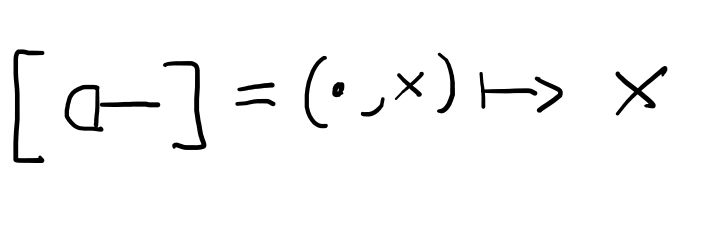
\includegraphics[width=0.75\linewidth]{../images/GLP/NewGenerator.png}
    \end{figure}
    together with the following axioms governing its interaction with
    the existing generators:
    \begin{figure}[H]
        \centering
        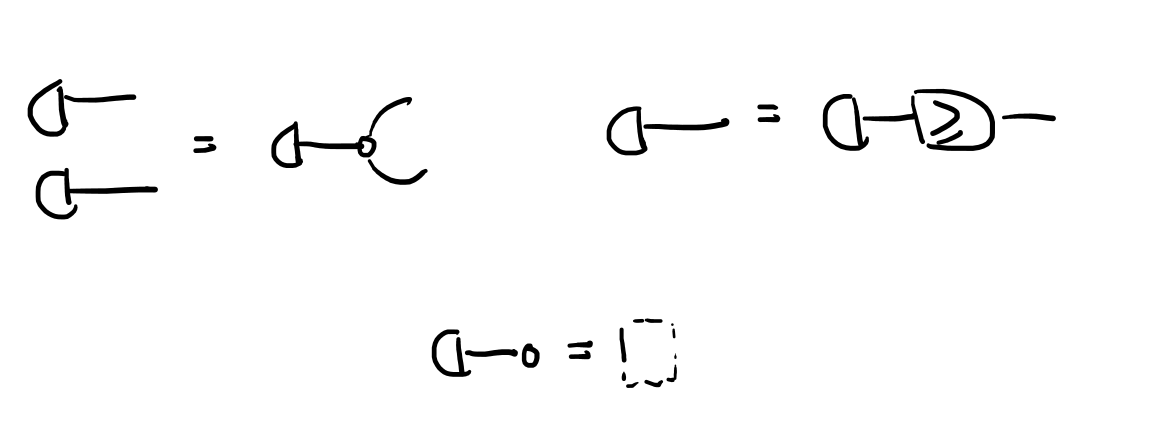
\includegraphics[width=0.75\linewidth]{../images/GLP/NewAxioms.png}
    \end{figure}
\end{definition}

The axioms represent expected properties of the linear cost function.
The one on the left expresses the linear property $f(x) + f(y) = f(x+y)$.
Observe that $f$ is the interpretation of the $\mushroom$ and the
sum denotes the vertical composition; composing two $\mushroom$ vertically
(adding) is the same as adding the wires in a single $\mushroom$. In turn, the
equation on the right expresses the fundamental property of
minimization, the infimum of any quantity lies in its lower bound:
\[\inf_x \{ x \mid x \ge y \} =  y.\]
Finally, the axiom in the middle is
the tautological case $\inf 0 = 0$.

\begin{definition}
    We call $\mathrm{FreeP}_{\mathbf{GLP}}$ the PROP freely generated
    by $\mathbf{GLP}$.
\end{definition}

The normal form theorem for $\mathbf{GLP}$ extends the one for
$\mathbf{GPA}$: every diagram can be reduced to a $\mathbf{GPA}$ block
encoding the constraints, composed with the new generator encoding the
objective. The proof proceeds by structural induction, using the existing
normal form for $\mathbf{GPA}$ as the inductive base.

\begin{theorem}[Normal Form]\label{thm:NormalFormGLP}
    For every diagram $c \in \mathbf{GLP}$, there exists a diagram $c'$
    in normal form such that $c = c'$:
    \begin{figure}[H]
        \centering
        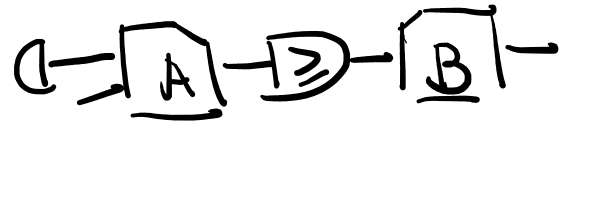
\includegraphics[width=0.75\linewidth]{../images/GLP/NormalForm.png}
    \end{figure}
    With $A$ and $b$ being an affine transformation, namely:
    \begin{figure}[H]
        \centering
        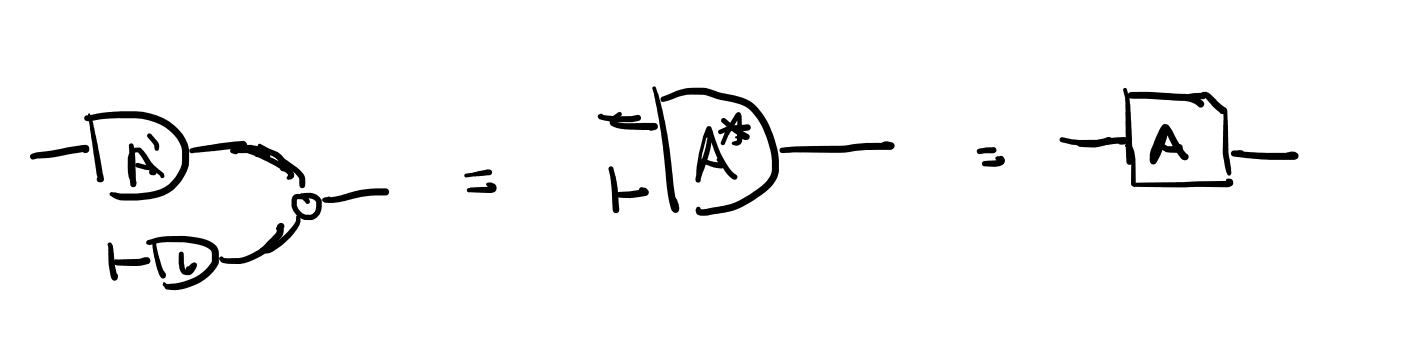
\includegraphics[width=0.75\linewidth]{../images/GLP/Affine transformation.png}
    \end{figure}
\end{theorem}

\begin{proof}
    The proof is by structural induction. First we show the two base cases:
    \begin{itemize}
        \item The generator $\mushroom$
        \begin{figure}[H]
            \centering
            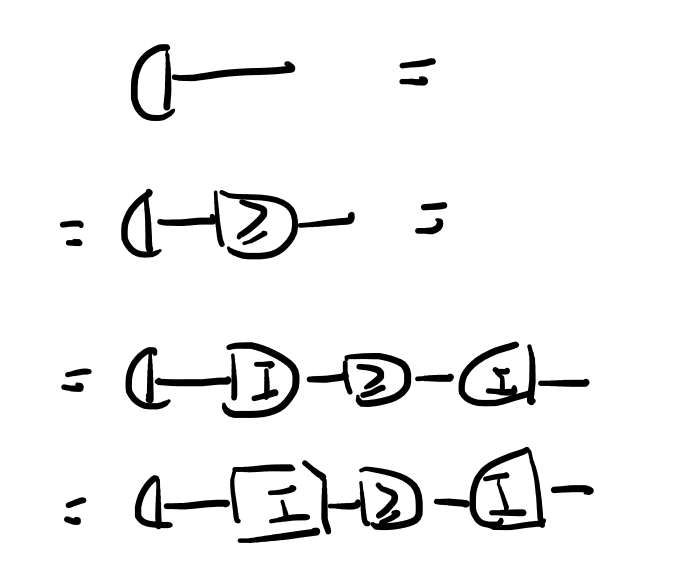
\includegraphics[width=0.75\linewidth]{../images/GLP/ProofNormalFOrm1.png}
        \end{figure}
        \item A diagram $c \in \textbf{GPA}$
        \begin{figure}[H]
            \centering
            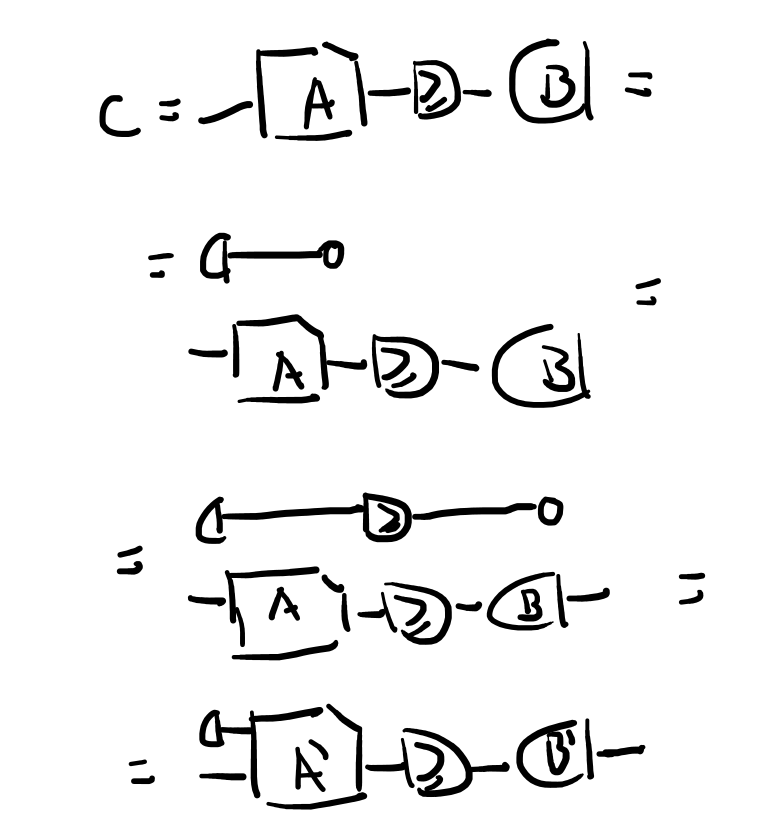
\includegraphics[width=0.75\linewidth]{../images/GLP/ProofNormalForm2.png}
        \end{figure}
    \end{itemize}
    For the inductive step, we verify that for any two diagrams
    $c, d \in \mathbf{GLP}$ satisfying the inductive hypothesis,
    both horizontal and vertical composition preserve the normal form.
    Closure under vertical composition follows immediately from the normal form.
    For horizontal composition, we apply Fourier-Motzkin Elimination in the \textbf{GLP}
    part of the diagram to recover the normal form.
\end{proof}

The following corollary reveals the geometric meaning of the normal form:
the $\mathbf{GPA}$ part of every $\mathbf{GLP}$ diagram encodes the
epigraph of the corresponding value function. This is the key structural
insight connecting the syntax to the semantic equivalence of
Proposition~\ref{prop:equalepi}.

\begin{corollary}[Epigraph Form]\label{cor:epigraph form}
    Given a diagram $d \in \mathbf{GLP}$ in normal form, it can always
    be rewritten as a diagram $d'$ of the form:
    \begin{figure}[H]
        \centering
        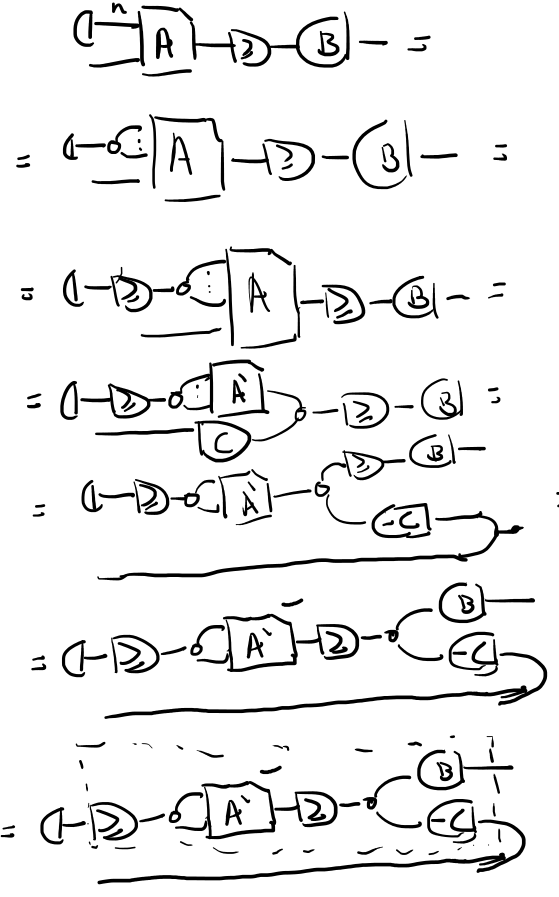
\includegraphics[width=1\linewidth]{../images/GLP/epiForm1.png}
    \end{figure}
    where the semantics of the dotted diagram is
    \[\left\{(t,y)\mid \exists\, x,\; A'x + a \ge [B\; -C]\, y,\; t\ge x,\; y =
    \begin{bmatrix} y_1 \\ y_2 \end{bmatrix}\right\}.\]
    This is the epigraph of the original diagram $d$
    \begin{align*}
        [d](y_1, y_2) &= \inf_{z} \; z \quad \text{s.t. } A z + a \ge B y_1 - C y_2 \\
        \mathrm{epi}([d]) &= \left\{(t, y_1, y_2) \mid \exists\, z \le t,\;
            A z + a \ge B y_1 - C y_2 \right\}
    \end{align*}
    such that $A = [A' \;C]$. We call this the \emph{epigraph form} of a linear program.
\end{corollary}

\section{Syntax-Semmantical Completeness}\label{sec:complete}

Fginally, we prove that our semmantics, namely that of Parametric Linear Programs, is fully axiomatize by the constrcuted SMT \textbf{GLP}. This sections divides in three parts:

\begin{itemize}
    \item Proving Soundness: a check that every
        generator is correctly interpreted and all our axioms
        are sound with the semmantics.
    \item Definibility: that every semmantical object, i.e. a
        \textit{Parametric Linear Program}, have a standard normal form and
        the latter is always the interpretation of some diagram in general form.
    \item Completeness: through the epigraph form, every two identical PLPs
        can be reduced to the same Polyhedral, which in turn makes the diagrams equal.
\end{itemize}

being those the necessary condition to show that the semmantic is fully axiomatized.

\begin{lemma}[Soundness]
   If $s = t$ in $\mathrm{FreeP}_{\mathbf{GLP}}$, then $[s] = [t]$
   in $\mathbf{PolyFun}$.
\end{lemma}

\begin{proof}
    All axioms inherited from $\mathbf{GPA}$ are already sound by the
    results of the previous section. It suffices to verify that the new
    axioms involving the LP generator preserve the semantics, which
    follows by direct computation:
    \begin{figure}[H]
        \centering
        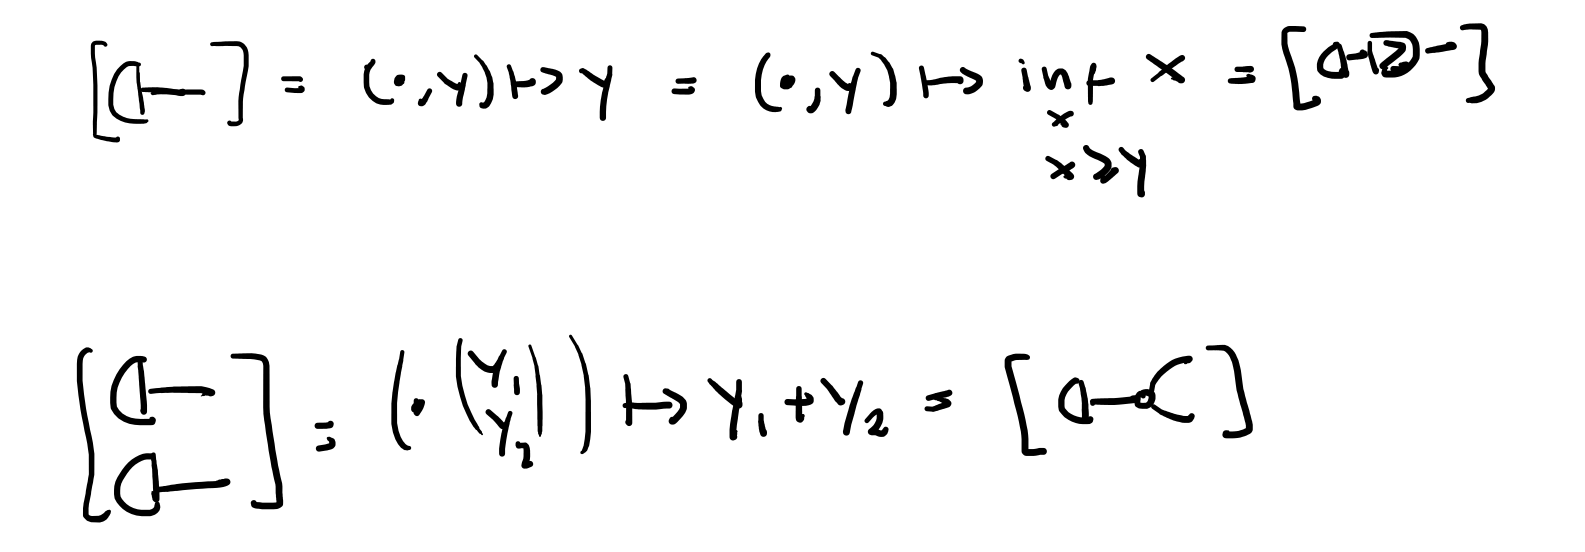
\includegraphics[width=0.75\linewidth]{../images/GLP/Soundness.png}
    \end{figure}
\end{proof}

\begin{lemma}[Definability / Expressivity]
    For every $f : m \to n$ in $\mathbf{PolyFun}$ there exists a
    $\Sigma$-term $s : m \to n$ in
    $\mathrm{Hom}_{\mathrm{FreeP}_{\mathbf{GLP}}}(m,n)$
    such that $[s] = f$.
\end{lemma}

\begin{proof}
    Since every polyhedral function is the maximum of a finite family of
    affine functions, it suffices to show that every piecewise affine
    convex function is expressible in $\mathbf{GLP}$. For an arbitrary
    such function $f(y) = \max_i R_i(y)$, where $\{R_i\}_{i=1,\dots,n}$
    is a family of affine functions, the following diagram provides the
    required syntactic representative:
    \begin{figure}[H]
        \centering
        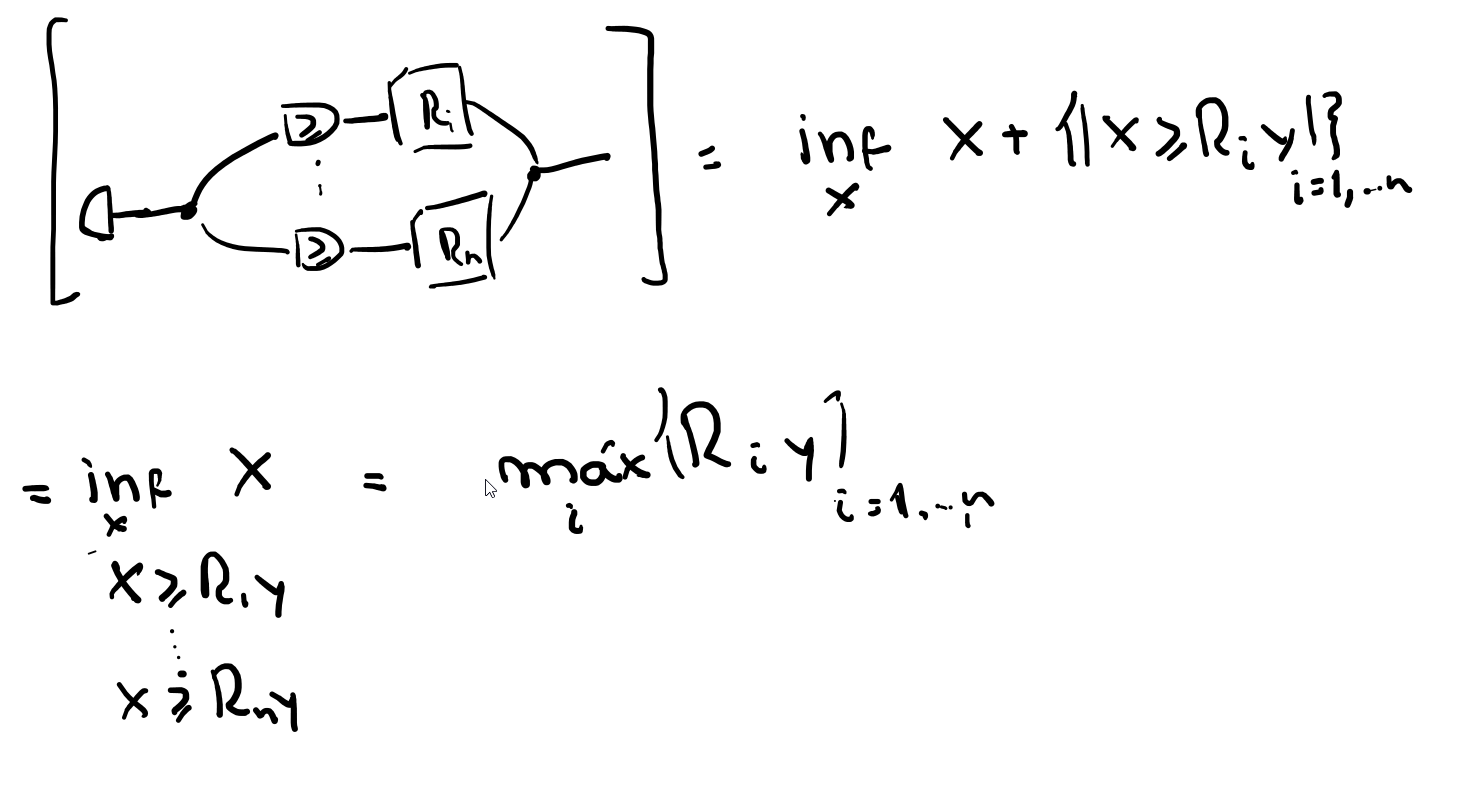
\includegraphics[width=0.75\linewidth]{../images/GLP/ExpressivityGLP.png}
    \end{figure}
\end{proof}

The final result is the completeness theorem for
$\mathbf{GLP}$. The proof brings together all the main tools developed
throughout: the epigraph form of Corollary~\ref{cor:epigraph form}, the
shared epigraph property of Proposition~\ref{prop:equalepi}, the
completeness of $\mathbf{GPA}$, and the FME-based normal form. We state
it subject to the completeness of the $\mathbf{GPA}$
polyhedra case (Theorem~\ref{thm:gpapresent}), which the argument appeals to;
subject to that result, the argument below goes through.

\begin{lemma}[Completeness]
   If $[c] = [d]$ in $\mathbf{PolyFun}$, then $c = d$ in
   $\mathrm{FreeP}_{\mathbf{GLP}}$.
\end{lemma}

\begin{proof}
    Let $v_1 = [c]$ and $v_2 = [d]$. By assumption $v_1 = v_2$, so
    Proposition~\ref{prop:equalepi} gives
    $\mathrm{epi}(v_1) = \mathrm{epi}(v_2) =: E$.

    By Corollary~\ref{cor:epigraph form}, both $c$ and $d$ admit
    epigraph forms $c = \mushroom ; c^*$ and $d = \mushroom ; d^*$
    with $[c^*] = [d^*] = E$ in $\mathbf{PolyRel}$:
    \begin{figure}[H]
        \centering
        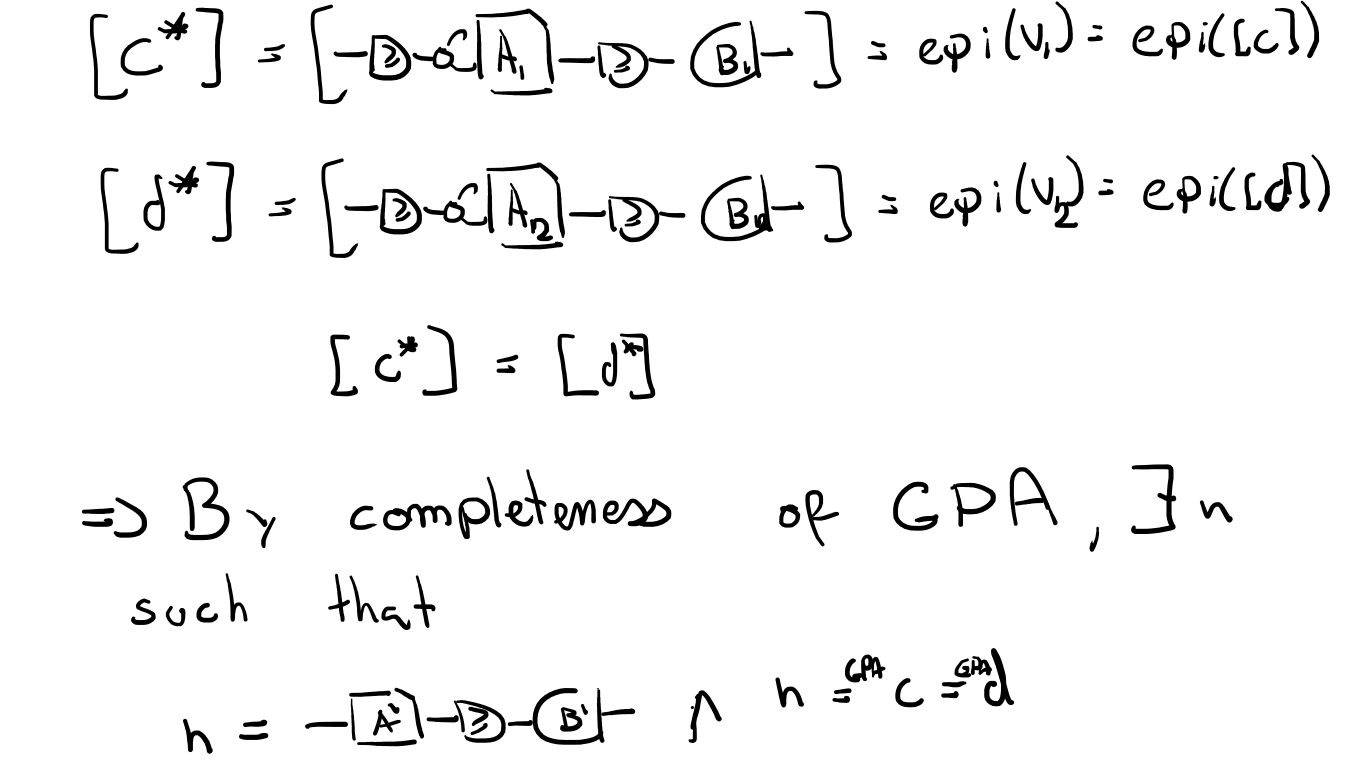
\includegraphics[width=0.75\linewidth]{../images/GLP/proofCompleteness1.png}
    \end{figure}
    Since $[c^*] = [d^*]$ in $\mathbf{PolyRel}$, completeness of
    $\mathbf{GPA}$ gives $c^* = d^*$ in
    $\mathrm{FreeP}_{\mathbf{GPA}}$. Therefore,
    \[
    c = \mushroom ; c^* = \mushroom ; d^* = d,
    \]
    as witnessed diagrammatically by:
    \begin{figure}[H]
        \centering
        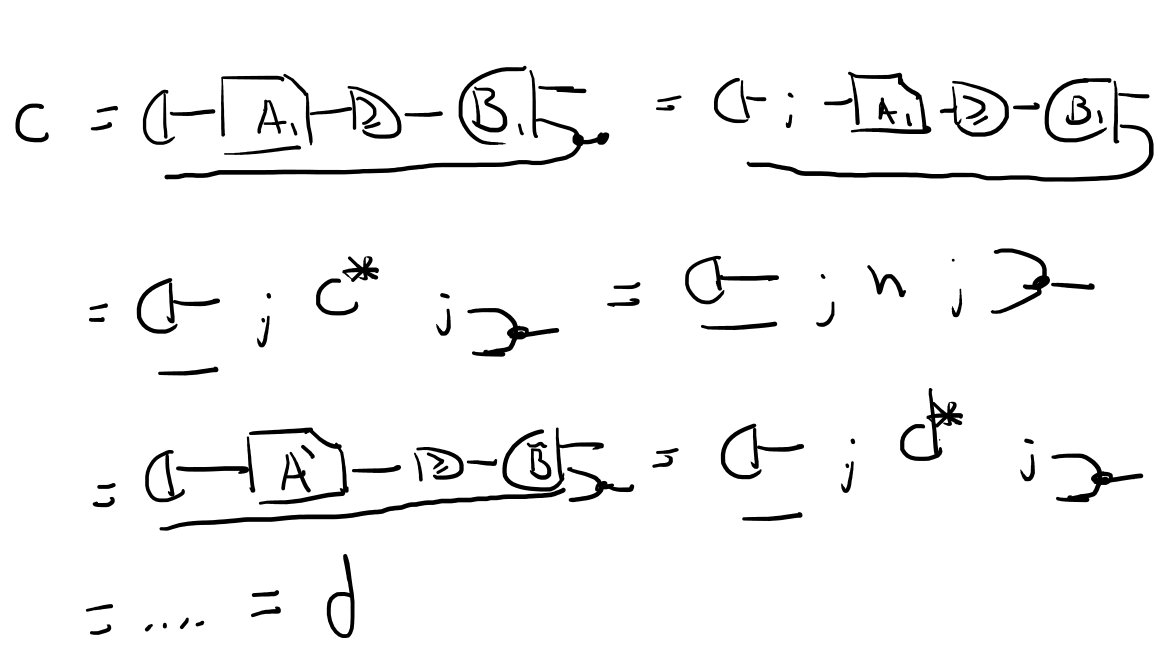
\includegraphics[width=0.75\linewidth]{../images/GLP/proofCompleteness4.png}
    \end{figure}
\end{proof}

As a consequence of the three lemmas above:

\begin{theorem}
    $\mathbf{LPRel}$ and $\mathbf{PolyFun}$ are both presented by $\mathrm{FreeP}_{\mathbf{GLP}}$.
\end{theorem}
\begin{proof}
    By the preceding three lemmas.
\end{proof}

\section{Discussion and Future Work}

We have built, through the addition of one generator and three axioms,
an elegant and complete diagrammatical theory for Parametric Linear Programming.
We argue that such a result not only unlocks a new way to interact with LP problems in an algebraic
and computational way, but also provides a new perspective on optimization through the lens of
a compositional framework. Optimization, namely LP problems, is lifted above
the setting of functional thinking and achieves a new status as a relational-theoretic
field embedded into the Extended-Lawvere Quantale category.

The development followed a strict linear discipline, adding exactly one new
generator at a time and verifying at each step that the resulting algebra is
sound, expressive, and complete with respect to a precisely defined semantic
category. The fact that such a linear development is
possible --- that each new class of optimization problems requires only a single
additional generator and a finite set of axioms --- is evidence that the
compositional structure is not imposed artificially but is genuinely present in
the mathematics. Polyhedral relations and quadratic relations are not merely two
classes of optimization problems that happen to admit graphical representations;
they are parallel enrichments of the same underlying affine structure, each adding
a different kind of expressive power, and their common base is a theorem rather than
an accident of notation.

The $\mathbf{GLP}$ theory has a natural extension to an even more expressive theory
when enriched with the gray arrow generator from $\mathbf{GQA}$. We believe that the class
of quadratic programs could be, just as was done in this work, fully axiomatized by such a
broader SMT. Another direction is the exploration of the functoriality of the bifunction
adjoint (the Legendre--Fenchel transform extended to morphisms)~\cite{willerton2015legendre, touchette2005legendre}: this suggests a duality theory
analogous to LP duality should be expressible diagrammatically as well.

A more applied direction concerns the computational implications of diagrammatic
normal forms. If two optimization problems are equal as morphisms in
$\mathbf{LPRel}$ if and only if their diagrams are related by the rewriting rules
of $\mathbf{GLP}$, then diagram simplification is problem simplification: a
rewriting system on string diagrams is simultaneously a symbolic preprocessor
for optimization solvers. Such an application of graphical algebras for theorem
solvers was already pointed to in other works \cite{bonchi2021.9farkas,bonchi2021polyhedral}.
This work has taken the first step on the road to fully expressing optimization within
its own algebraic setting.

\printbibliography
\end{document}
